\documentclass[[../main.tex]{subfiles}

\begin{document}

\section{Resultados obtenidos}

Los resultados aquí presentados se han realizado utilizando el sistema ampliador de resolución (EnhanceNet) y con las versiones (del sistema principal) 1.0\textunderscore 256b en el caso de Monet y Cézanne, y 1.0\textunderscore 256 en el caso de Van Gogh. Dichas versiones implementan la arquitectura resnet y utilizan el archivo de configuración \textit{configuracion\textunderscore 256.json} suministrado en el anexo \ref{anexo:archivos_configuracion}.

\subsection{Paso de fotografías a cuadros}
\subsubsection{Paisajes del dataset}
    \paragraph{Cézanne}
        \begin{figure}[!htb]
            \begin{subfigure}[b]{0.49\textwidth}
            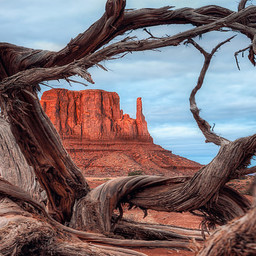
\includegraphics[width=0.65\textwidth]{imagenes/imagen2cuadro/dataset/cezanne/2014-08-06 08_56_57.jpg}
            \end{subfigure}
        \hfill
            \begin{subfigure}[b]{0.49\textwidth}
            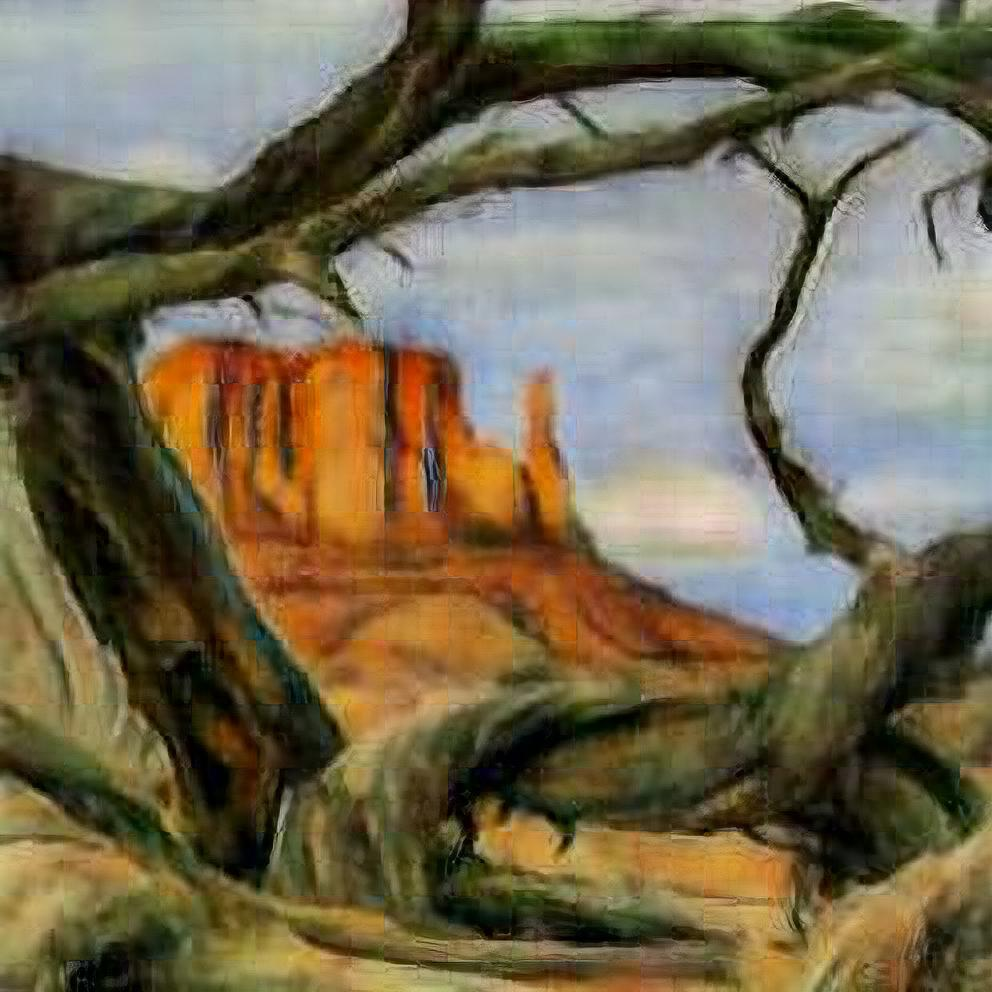
\includegraphics[width=0.65\textwidth]{imagenes/imagen2cuadro/dataset/cezanne/2014-08-06 08_56_57_2.jpg}
            \end{subfigure}
        \caption{Cuadro de Cézanne generado en el desierto}
        \label{fig:cezanne_cuadro_dataset_desierto}
        \end{figure}
        
        \begin{figure}[!htb]
            \begin{subfigure}[b]{0.49\textwidth}
            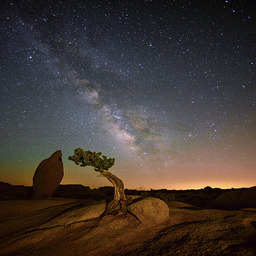
\includegraphics[width=0.65\textwidth]{imagenes/imagen2cuadro/dataset/cezanne/2014-08-09 00_16_45.jpg}
            \end{subfigure}
        \hfill
            \begin{subfigure}[b]{0.49\textwidth}
            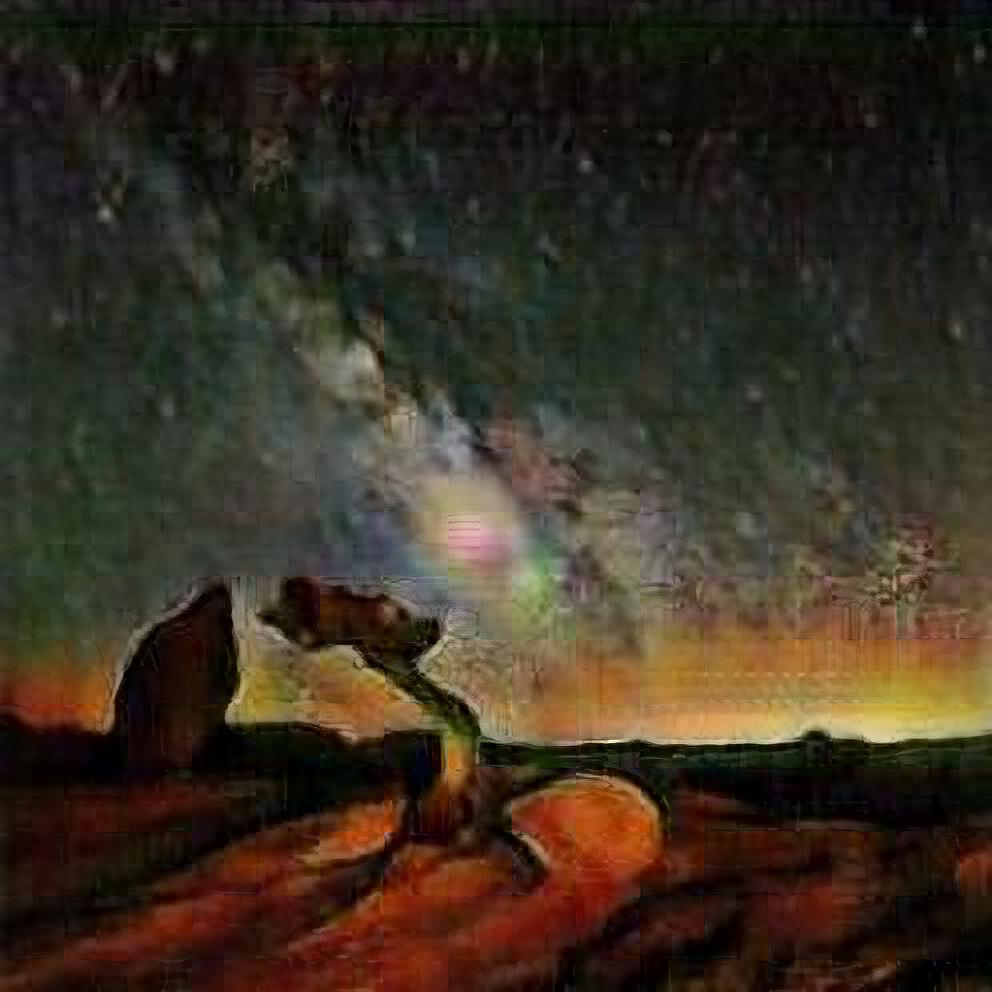
\includegraphics[width=0.65\textwidth]{imagenes/imagen2cuadro/dataset/cezanne/2014-08-09 00_16_45_2.jpg}
            \end{subfigure}
        \caption{Cuadro de Cézanne generado en la noche}
        \label{fig:cezanne_cuadro_dataset_noche}
        \end{figure}
        
        \begin{figure}[!htb]
            \begin{subfigure}[b]{0.49\textwidth}
            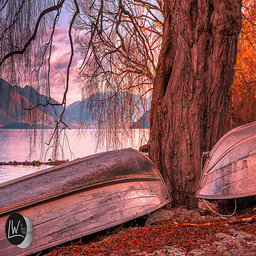
\includegraphics[width=0.65\textwidth]{imagenes/imagen2cuadro/dataset/cezanne/2014-08-25 17_36_12.jpg}
            \end{subfigure}
        \hfill
            \begin{subfigure}[b]{0.49\textwidth}
            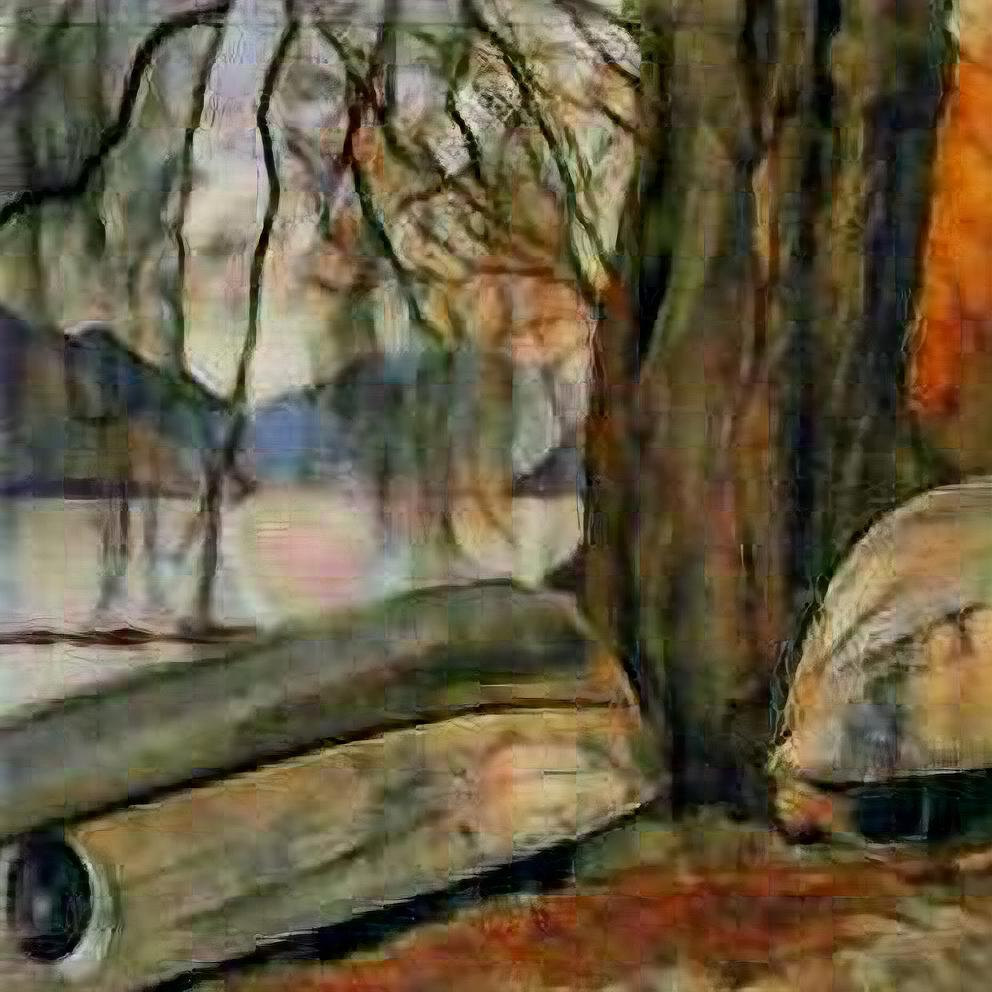
\includegraphics[width=0.65\textwidth]{imagenes/imagen2cuadro/dataset/cezanne/2014-08-25 17_36_12_2.jpg}
            \end{subfigure}
        \caption{Cuadro de Cézanne generado en una orilla}
        \label{fig:cezanne_cuadro_dataset_orilla}
        \end{figure}
        
        \begin{figure}[!htb]
            \begin{subfigure}[b]{0.49\textwidth}
            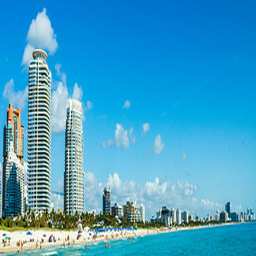
\includegraphics[width=0.65\textwidth]{imagenes/imagen2cuadro/dataset/cezanne/2015-04-06 20_32_26.jpg}
            \end{subfigure}
        \hfill
            \begin{subfigure}[b]{0.49\textwidth}
            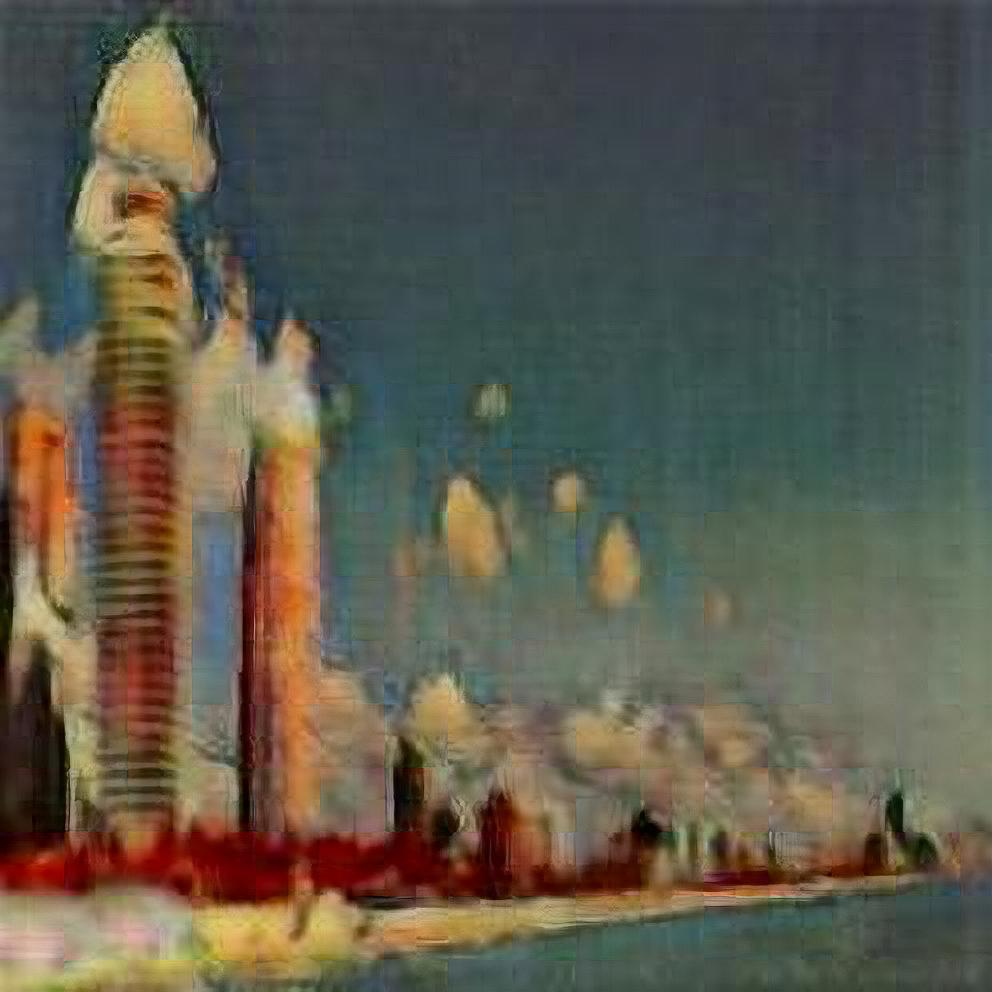
\includegraphics[width=0.65\textwidth]{imagenes/imagen2cuadro/dataset/cezanne/2015-04-06 20_32_26_2.jpg}
            \end{subfigure}
        \caption{Cuadro de Cézanne generado de unos edificios}
        \label{fig:cezanne_cuadro_dataset_edificios}
        \end{figure}
        
        En este caso puede verse a simple vista cómo ha aprendido el sistema la rojiza paleta de colores característica de Cézanne, además de los cielos. En el caso de la figura \ref{fig:cezanne_cuadro_dataset_noche} puede verse como la parte de luz ha sido exagerada por el modelo, debido a que no ha recibido apenas entrenamiento en imágenes nocturnas.
        
        \newpage

    \paragraph{Monet}
    
    \begin{figure}[!htb]
            \begin{subfigure}[b]{0.49\textwidth}
            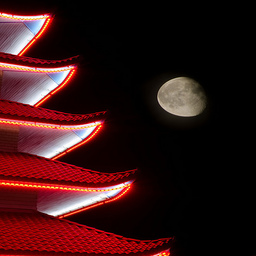
\includegraphics[width=0.65\textwidth]{imagenes/imagen2cuadro/dataset/monet/2014-08-06 15_33_46.jpg}
            \end{subfigure}
        \hfill
            \begin{subfigure}[b]{0.49\textwidth}
            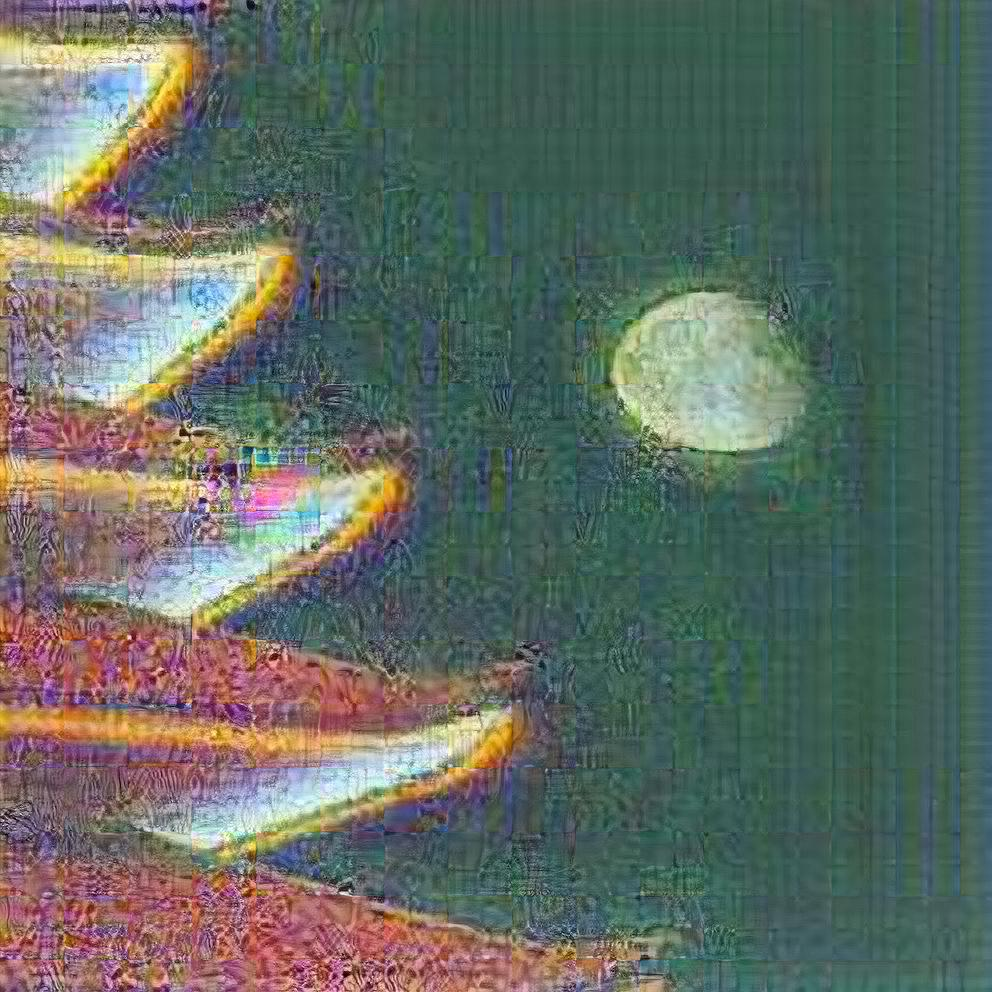
\includegraphics[width=0.65\textwidth]{imagenes/imagen2cuadro/dataset/monet/2014-08-06 15_33_46_2.jpg}
            \end{subfigure}
        \caption{Cuadro de Monet generado a partir de un edificio japonés de noche}
        \label{fig:monet_cuadro_edificio_japones_noche}
        \end{figure}
        
        \begin{figure}[!htb]
            \begin{subfigure}[b]{0.49\textwidth}
            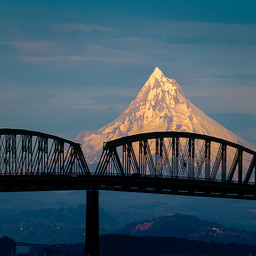
\includegraphics[width=0.65\textwidth]{imagenes/imagen2cuadro/dataset/monet/2014-08-07 21_31_39.jpg}
            \end{subfigure}
        \hfill
            \begin{subfigure}[b]{0.49\textwidth}
            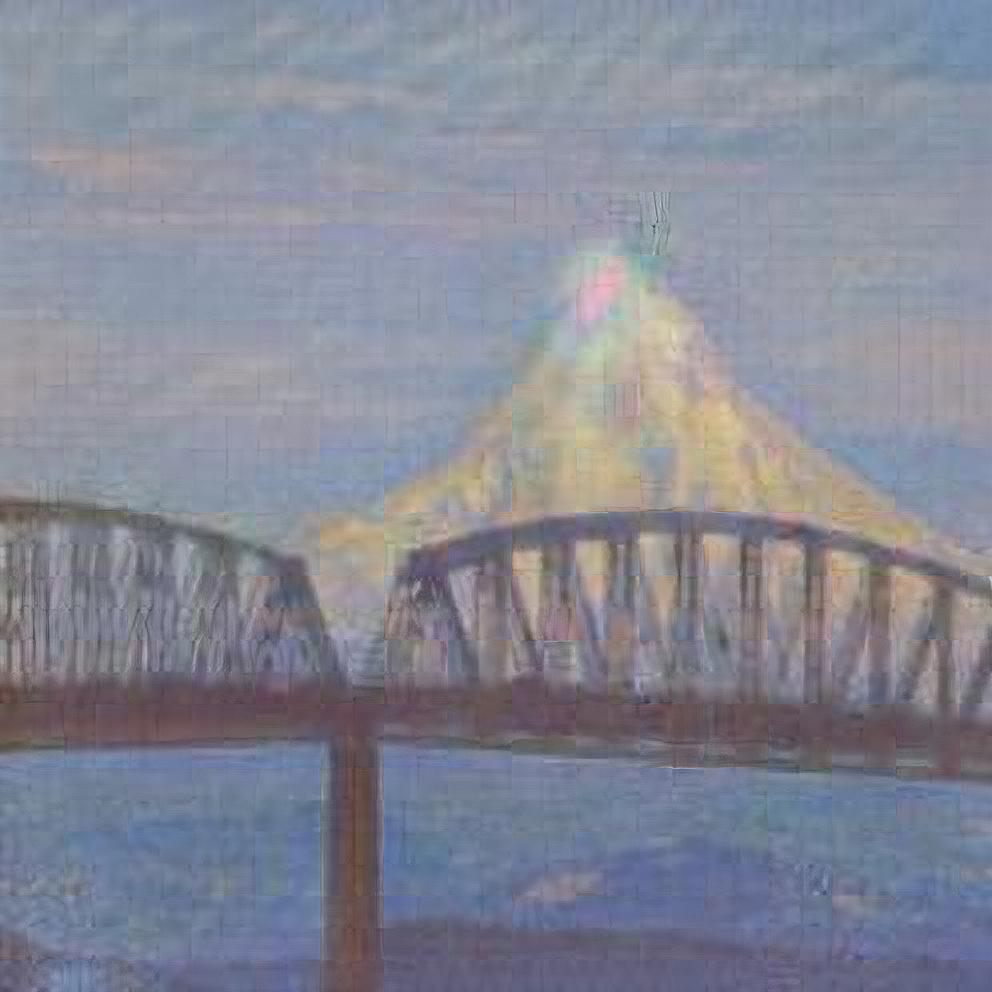
\includegraphics[width=0.65\textwidth]{imagenes/imagen2cuadro/dataset/monet/2014-08-07 21_31_39_2.jpg}
            \end{subfigure}
        \caption{Cuadro de Monet generado a partir de un puente}
        \label{fig:monet_cuadro_puente}
        \end{figure}
        
        \begin{figure}[!htb]
            \begin{subfigure}[b]{0.49\textwidth}
            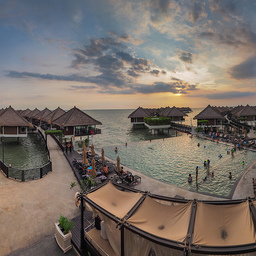
\includegraphics[width=0.65\textwidth]{imagenes/imagen2cuadro/dataset/monet/2014-08-15 08_48_43.jpg}
            \end{subfigure}
        \hfill
            \begin{subfigure}[b]{0.49\textwidth}
            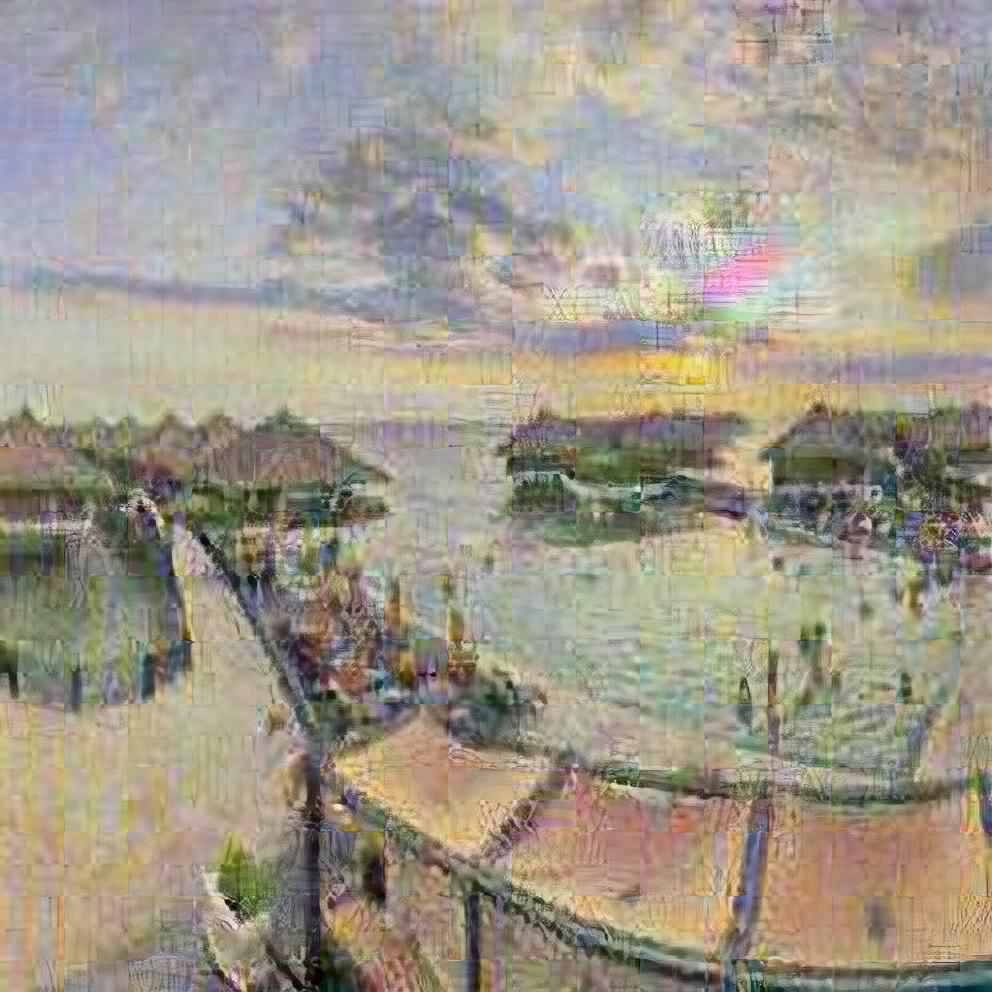
\includegraphics[width=0.65\textwidth]{imagenes/imagen2cuadro/dataset/monet/2014-08-15 08_48_43_2.jpg}
            \end{subfigure}
        \caption{Cuadro de Monet generado a partir de edificaciones en el agua}
        \label{fig:monet_cuadro_edificaciones_agua}
        \end{figure}
        
        \begin{figure}[!htb]
            \begin{subfigure}[b]{0.49\textwidth}
            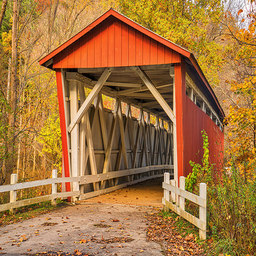
\includegraphics[width=0.65\textwidth]{imagenes/imagen2cuadro/dataset/monet/2014-10-24 04_26_01.jpg}
            \end{subfigure}
        \hfill
            \begin{subfigure}[b]{0.49\textwidth}
            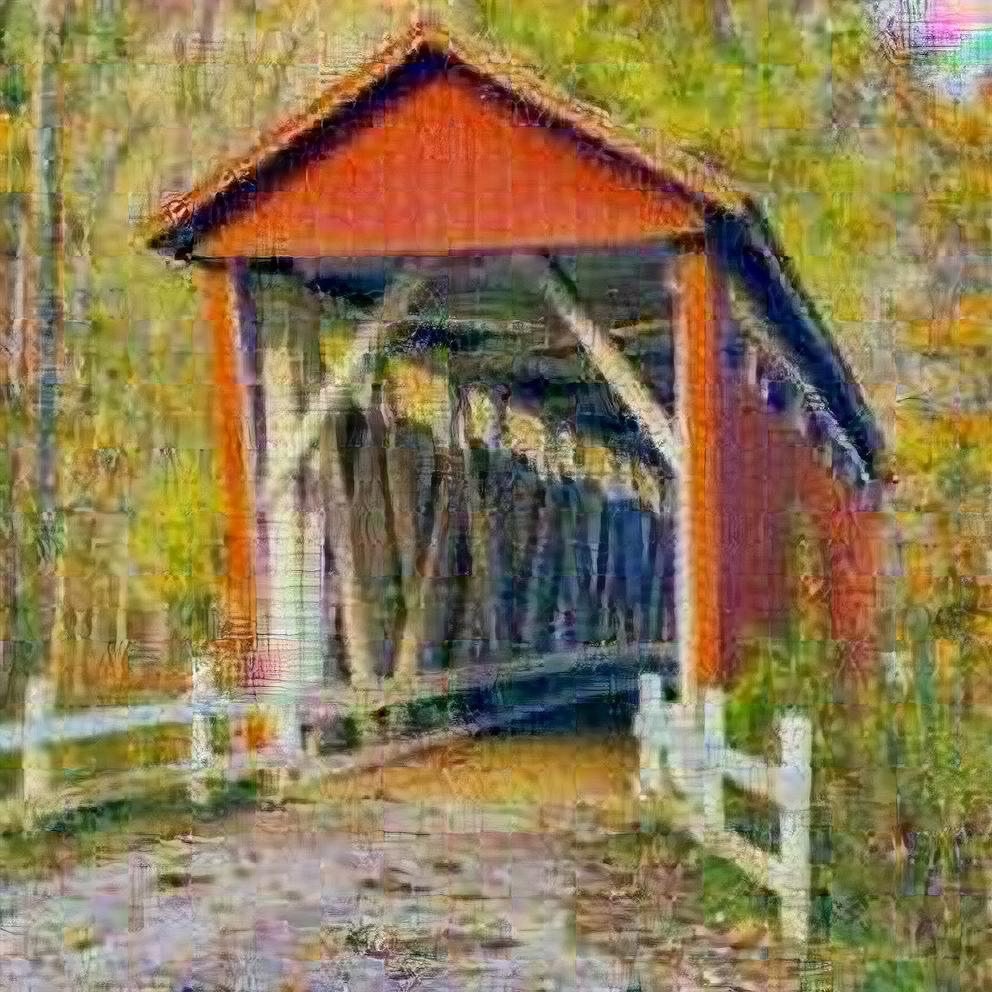
\includegraphics[width=0.65\textwidth]{imagenes/imagen2cuadro/dataset/monet/2014-10-24 04_26_01_2.jpg}
            \end{subfigure}
        \caption{Cuadro de Monet generado a partir de un puente de madera}
        \label{fig:monet_cuadro_puente_madera}
        \end{figure}
        
        Podemos ver a simple vista que el modelo ha interpretado los cuadros de Monet como aquellos con tonalidades azules frías. Es especialmente llamativo el caso de la figura \ref{fig:monet_cuadro_edificio_japones_noche}: el sistema \textit{blanquea} el cielo de la noche, nuevamente debido a la falta de ejemplos de cuadros nocturnos de Monet.
        
        \newpage
    
    \paragraph{Van Gogh}
        
        \begin{figure}[!htb]
            \begin{subfigure}[b]{0.49\textwidth}
            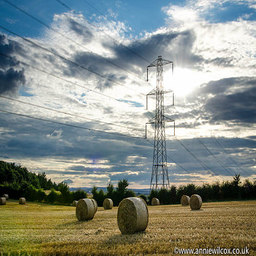
\includegraphics[width=0.65\textwidth]{imagenes/imagen2cuadro/dataset/vangogh/2014-08-05 09_28_38.jpg}
            \end{subfigure}
        \hfill
            \begin{subfigure}[b]{0.49\textwidth}
            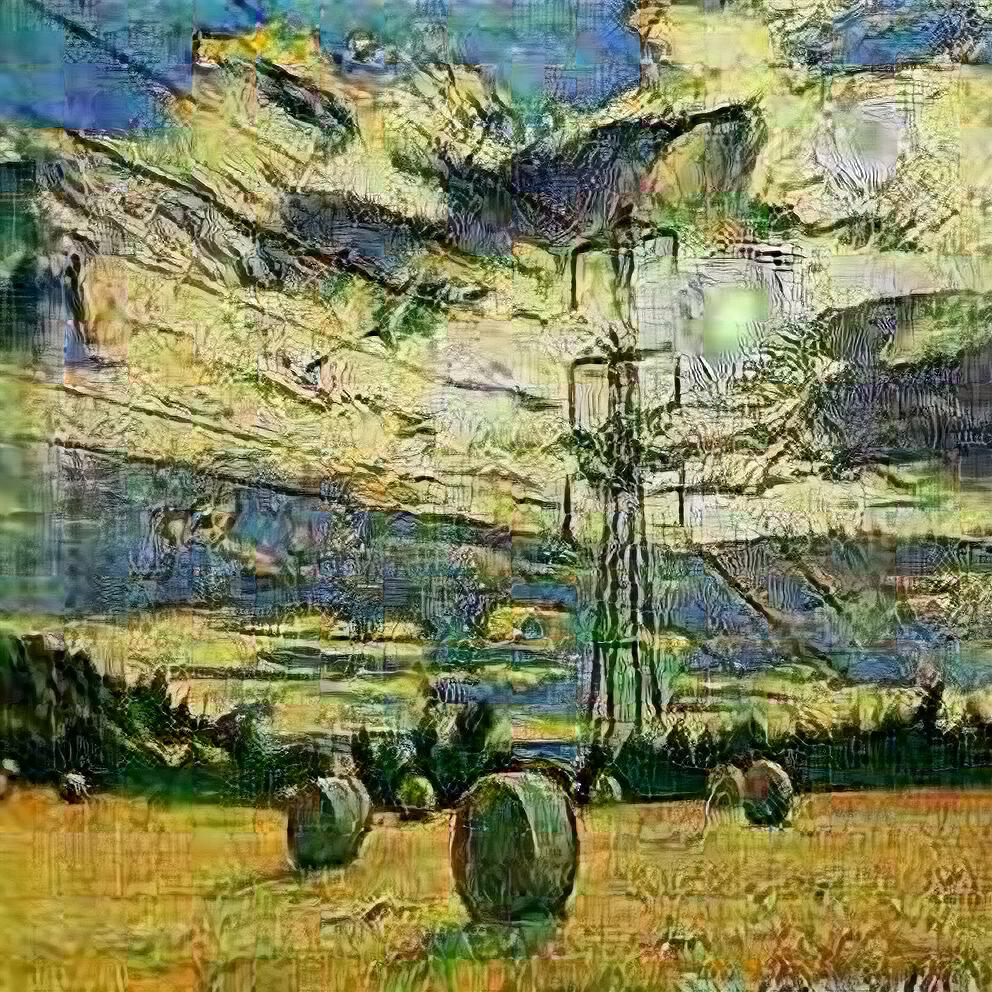
\includegraphics[width=0.65\textwidth]{imagenes/imagen2cuadro/dataset/vangogh/2014-08-05 09_28_38_2.jpg}
            \end{subfigure}
        \caption{Cuadro de Van Gogh generado a partir de un campo con bolas}
        \label{fig:vangogh_cuadro_campo_bolas}
        \end{figure}
        
        \begin{figure}[!htb]
            \begin{subfigure}[b]{0.49\textwidth}
            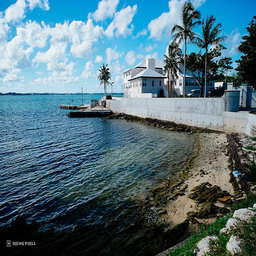
\includegraphics[width=0.65\textwidth]{imagenes/imagen2cuadro/dataset/vangogh/2014-08-18 17_24_39.jpg}
            \end{subfigure}
        \hfill
            \begin{subfigure}[b]{0.49\textwidth}
            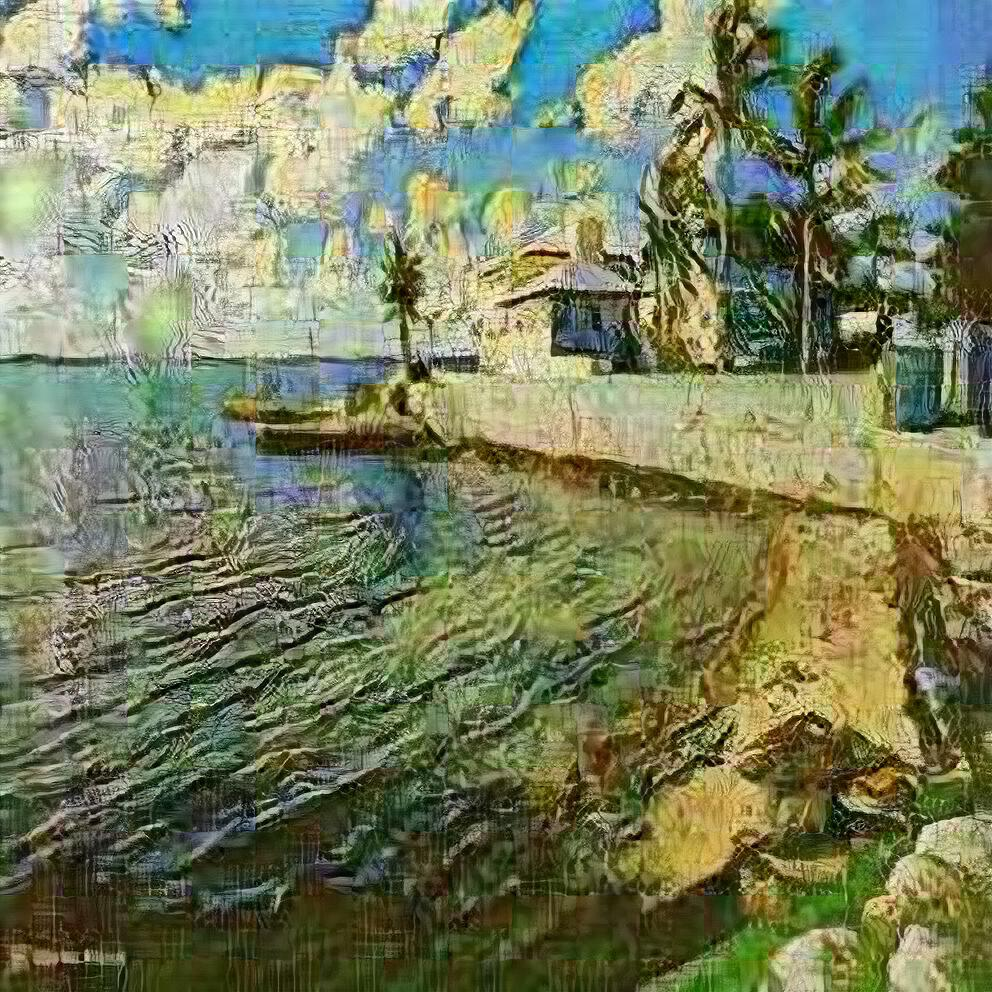
\includegraphics[width=0.65\textwidth]{imagenes/imagen2cuadro/dataset/vangogh/2014-08-18 17_24_39_2.jpg}
            \end{subfigure}
        \caption{Cuadro de Van Gogh generado a partir de una casa en el mar}
        \label{fig:vangogh_cuadro_casa_mar}
        \end{figure}
        
        \begin{figure}[!htb]
            \begin{subfigure}[b]{0.49\textwidth}
            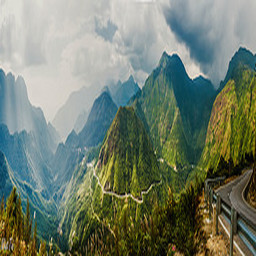
\includegraphics[width=0.65\textwidth]{imagenes/imagen2cuadro/dataset/vangogh/2014-08-20 08_13_24.jpg}
            \end{subfigure}
        \hfill
            \begin{subfigure}[b]{0.49\textwidth}
            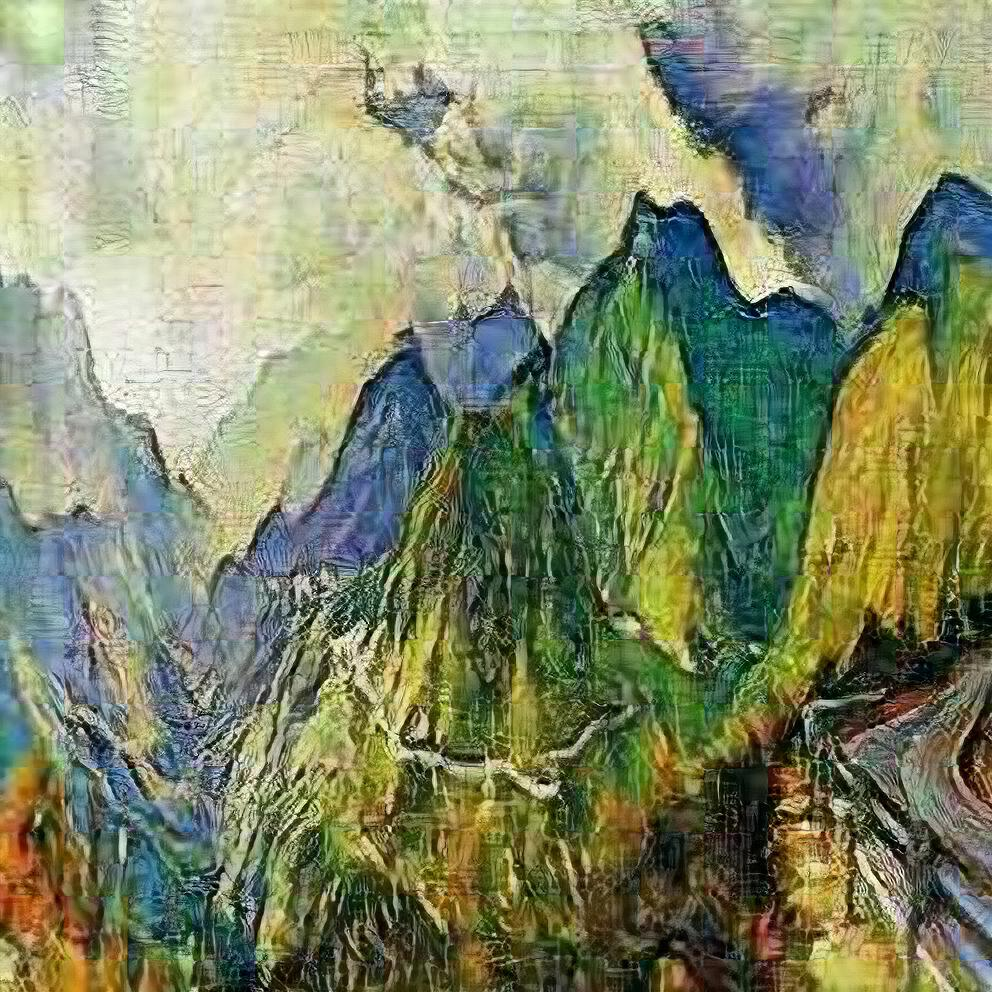
\includegraphics[width=0.65\textwidth]{imagenes/imagen2cuadro/dataset/vangogh/2014-08-20 08_13_24_2.jpg}
            \end{subfigure}
        \caption{Cuadro de Van Gogh generado a partir de una montaña}
        \label{fig:vangogh_cuadro_montaña_carretera}
        \end{figure}
        
        \begin{figure}[!htb]
            \begin{subfigure}[b]{0.49\textwidth}
            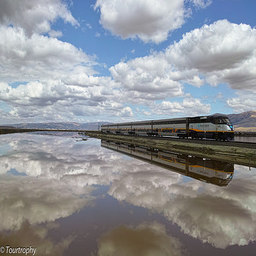
\includegraphics[width=0.65\textwidth]{imagenes/imagen2cuadro/dataset/vangogh/2014-09-18 14_23_57.jpg}
            \end{subfigure}
        \hfill
            \begin{subfigure}[b]{0.49\textwidth}
            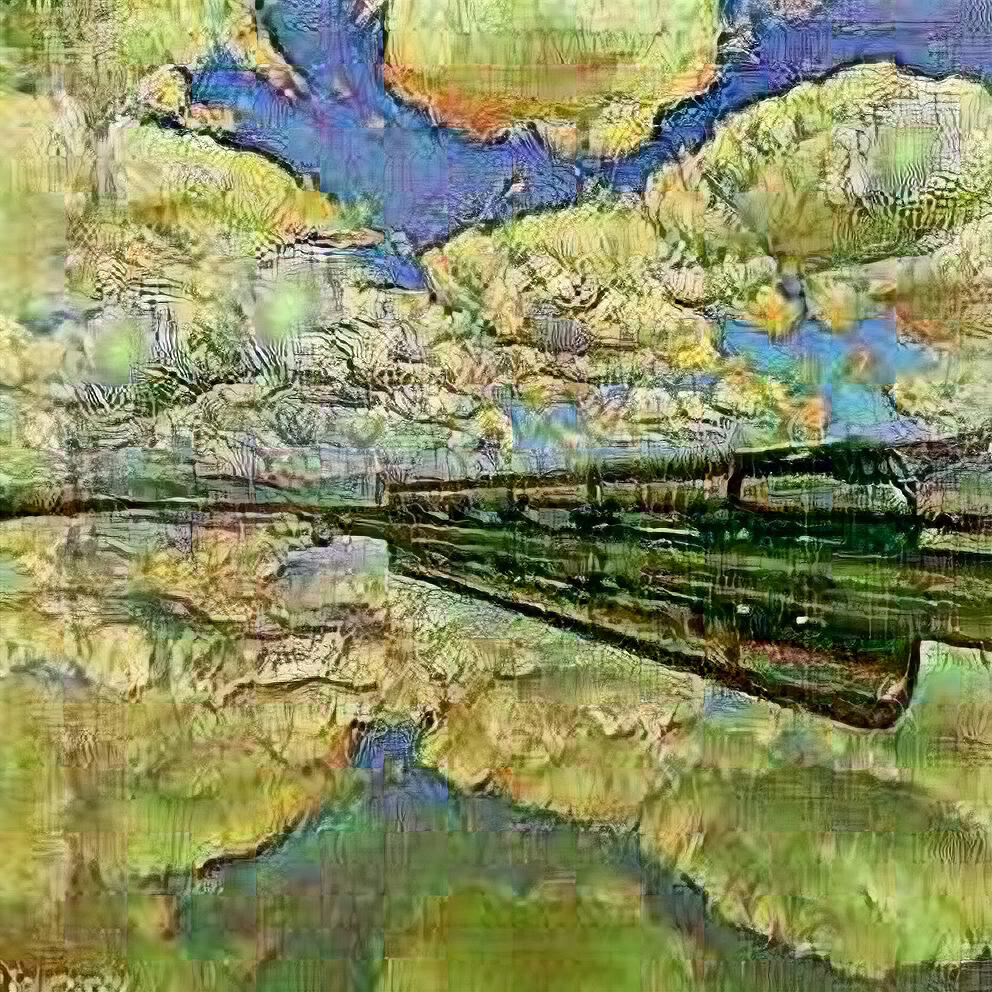
\includegraphics[width=0.65\textwidth]{imagenes/imagen2cuadro/dataset/vangogh/2014-09-18 14_23_57_2.jpg}
            \end{subfigure}
        \caption{Cuadro de Van Gogh a partir de un ferrocarril en el agua}
        \label{fig:vangogh_cuadro_tren_agua}
        \end{figure}
        
        En este caso pueden verse más diferencias más allá de las paletas de color: se ve fácilmente las pinceladas bruscas características de Van Gogh, dando una textura especial a los cuadros. 
        
        \newpage
    
\subsubsection{Fotos del autor}
    \paragraph{Cézanne}
        \begin{figure}[!htb]
            \begin{subfigure}[b]{0.49\textwidth}
            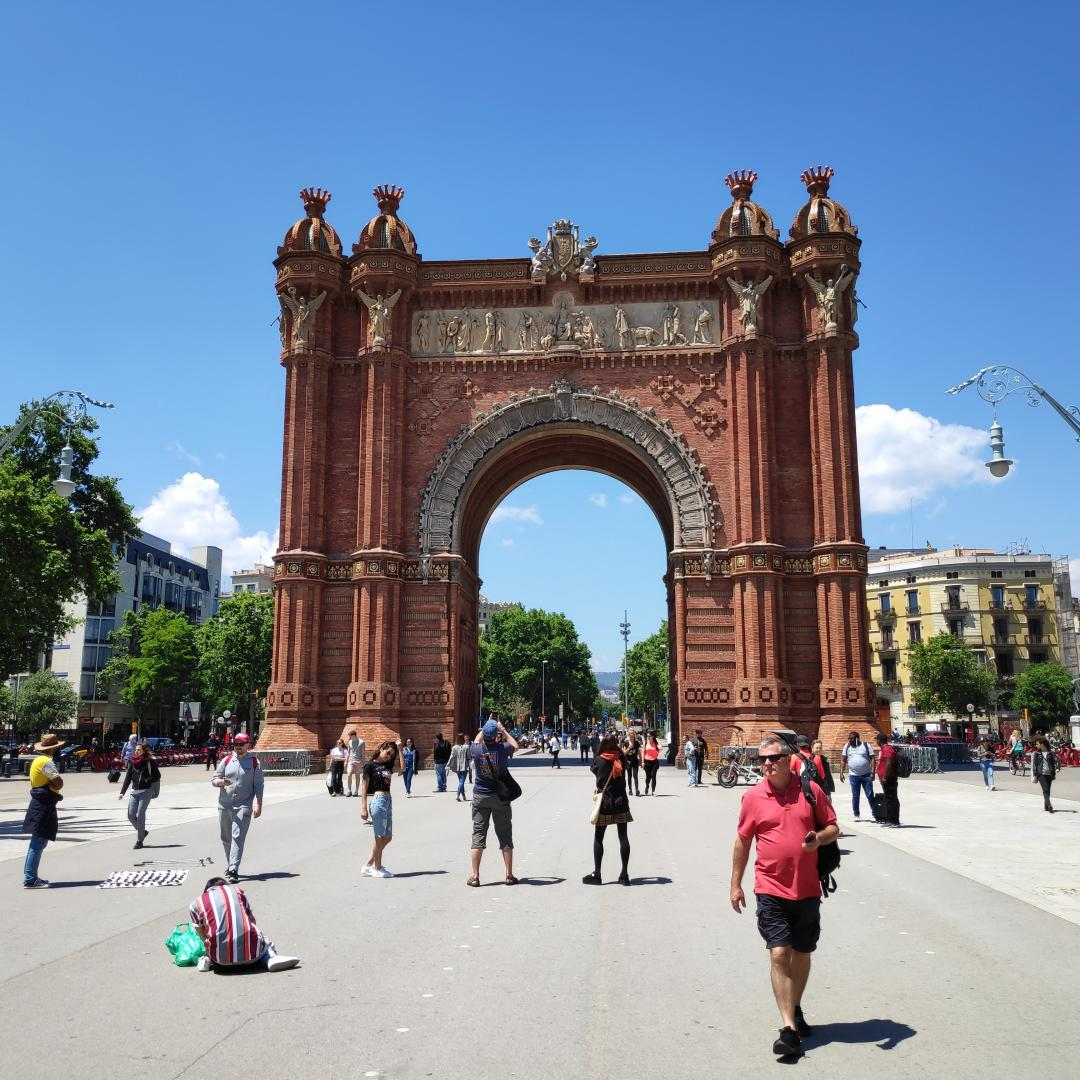
\includegraphics[width=0.65\textwidth]{imagenes/imagen2cuadro/propias/cezanne/IMG_20190520_141500.jpg}
            \end{subfigure}
        \hfill
            \begin{subfigure}[b]{0.49\textwidth}
            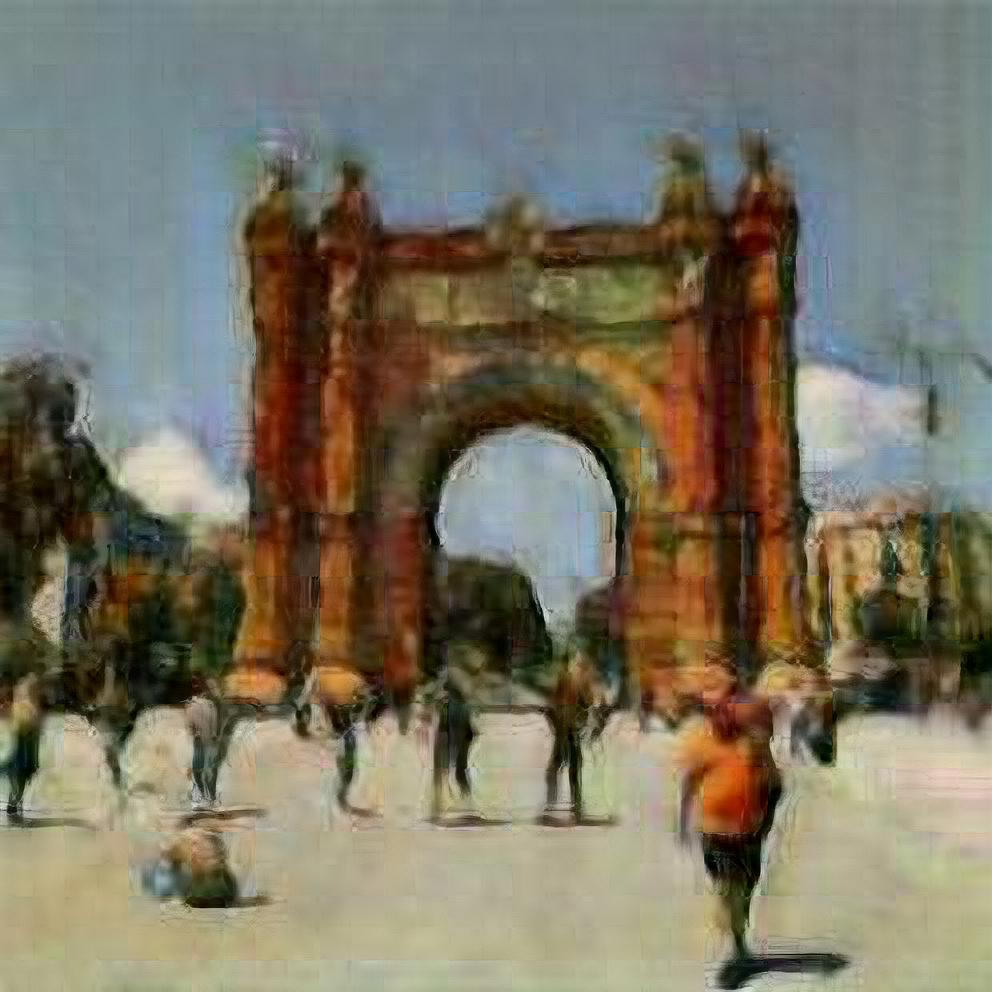
\includegraphics[width=0.65\textwidth]{imagenes/imagen2cuadro/propias/cezanne/IMG_20190520_141500_2.jpg}
            \end{subfigure}
        \caption{Cuadro de Cézanne generado en el arco del triunfo de Barcelona}
        \label{fig:cezanne_cuadro_arco_bcn}
        \end{figure}
        
        \begin{figure}[!htb]
            \begin{subfigure}[b]{0.49\textwidth}
            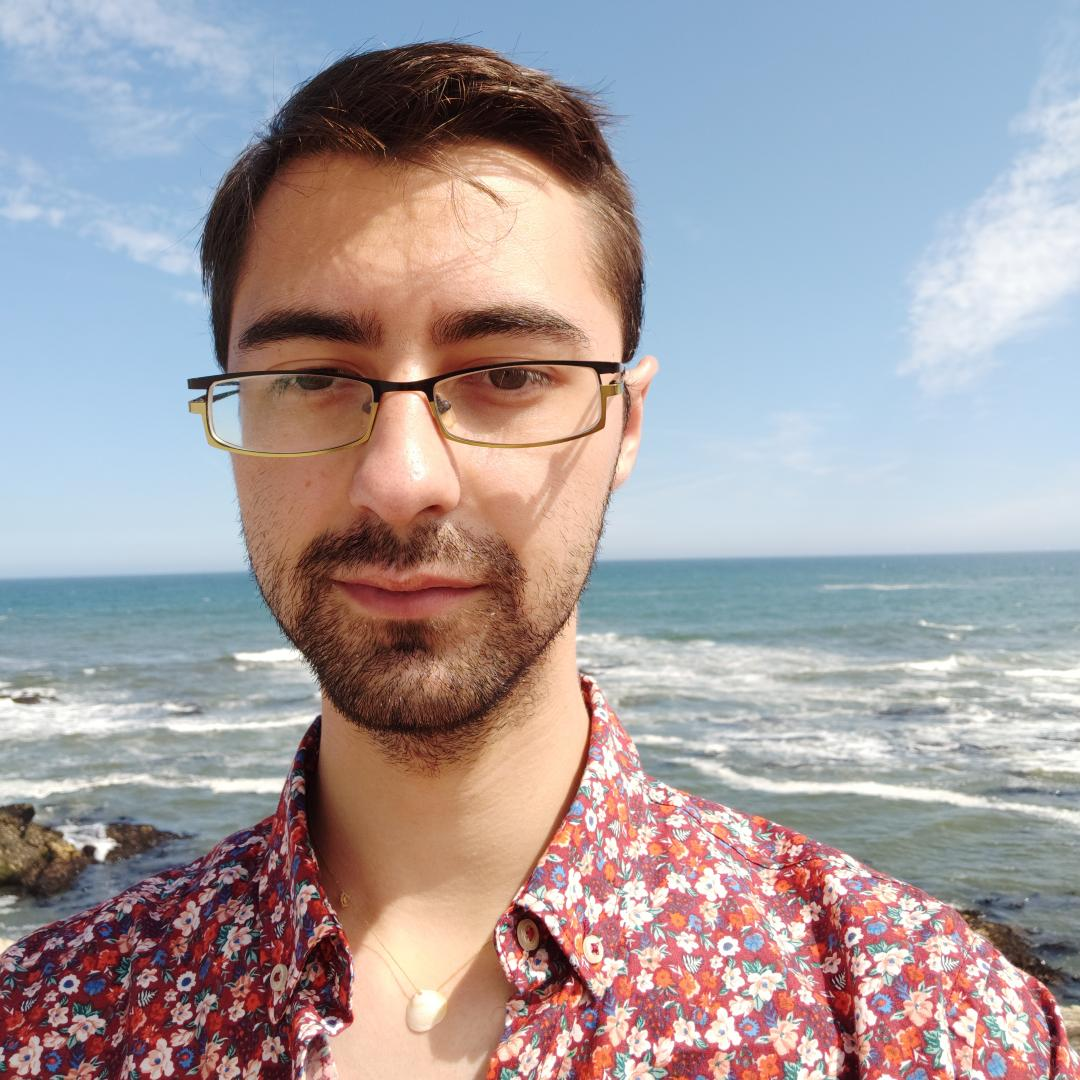
\includegraphics[width=0.65\textwidth]{imagenes/imagen2cuadro/propias/cezanne/IMG_20190901_131836.jpg}
            \end{subfigure}
        \hfill
            \begin{subfigure}[b]{0.49\textwidth}
            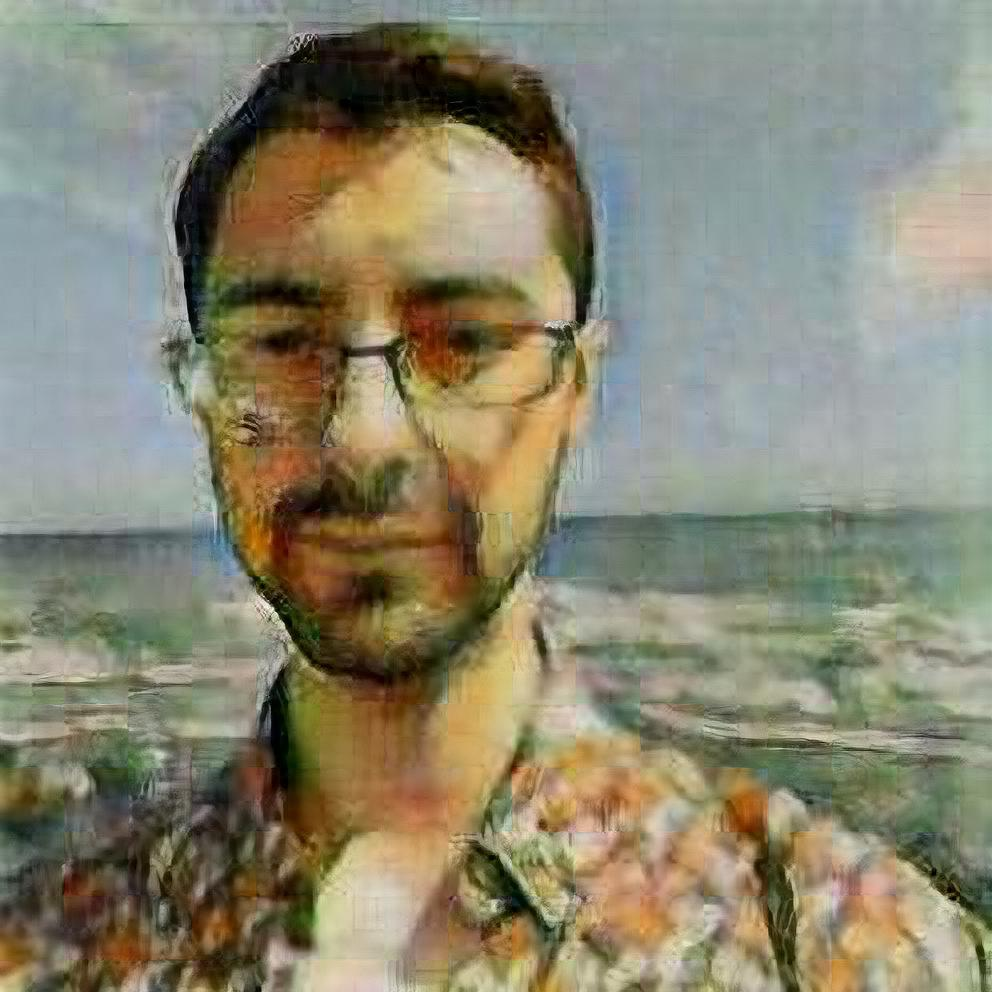
\includegraphics[width=0.65\textwidth]{imagenes/imagen2cuadro/propias/cezanne/IMG_20190901_131836_2.jpg}
            \end{subfigure}
        \caption{Cuadro de Cézanne generado a partir de una foto en una playa del autor}
        \label{fig:cezanne_cuadro_selfie_playa}
        \end{figure}
        
        \begin{figure}[!htb]
            \begin{subfigure}[b]{0.49\textwidth}
            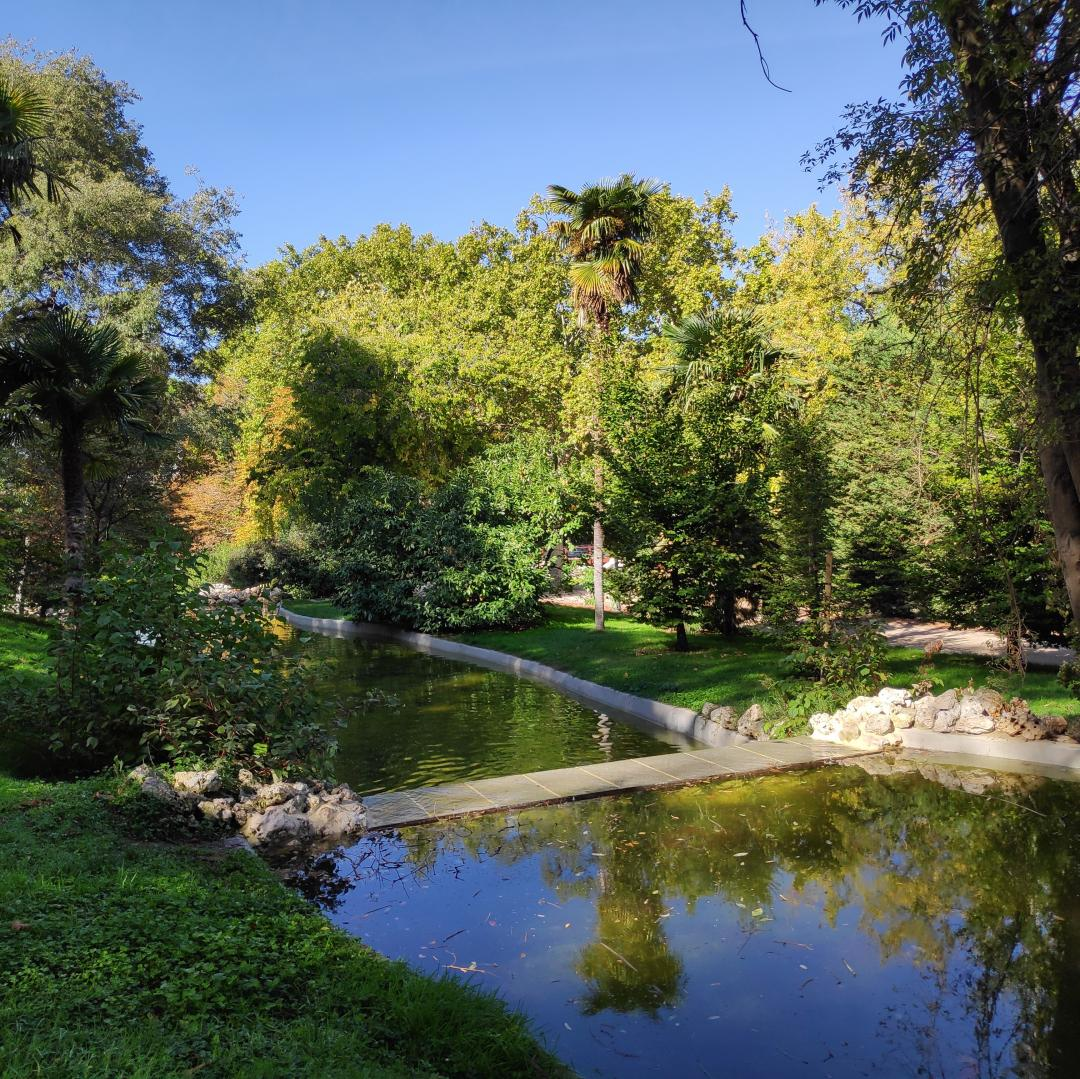
\includegraphics[width=0.65\textwidth]{imagenes/imagen2cuadro/propias/cezanne/IMG_20191026_123831_1.jpg}
            \end{subfigure}
        \hfill
            \begin{subfigure}[b]{0.49\textwidth}
            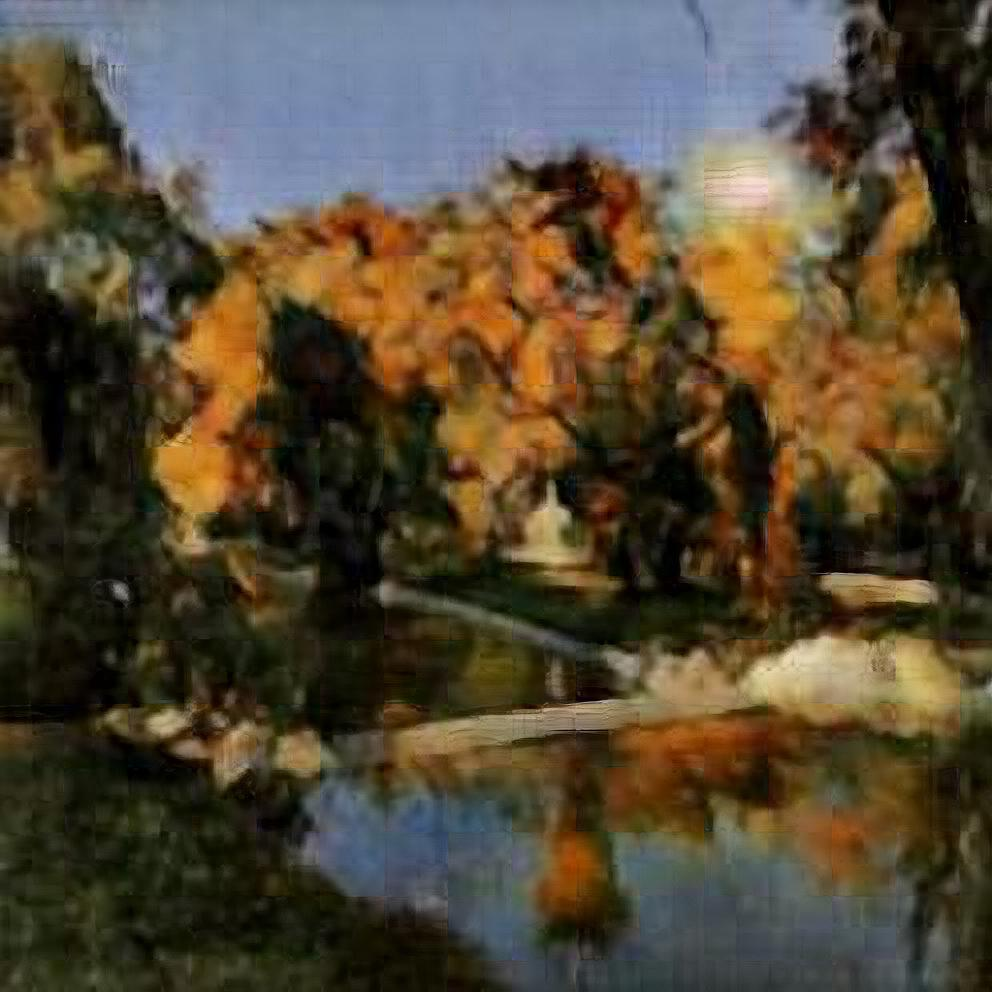
\includegraphics[width=0.65\textwidth]{imagenes/imagen2cuadro/propias/cezanne/IMG_20191026_123831_1_2.jpg}
            \end{subfigure}
        \caption{Cuadro de Cézanne generado de una foto de un parque de Madrid}
        \label{fig:cezanne_cuadro_parque_madrid}
        \end{figure}
        
        \begin{figure}[!htb]
            \begin{subfigure}[b]{0.49\textwidth}
            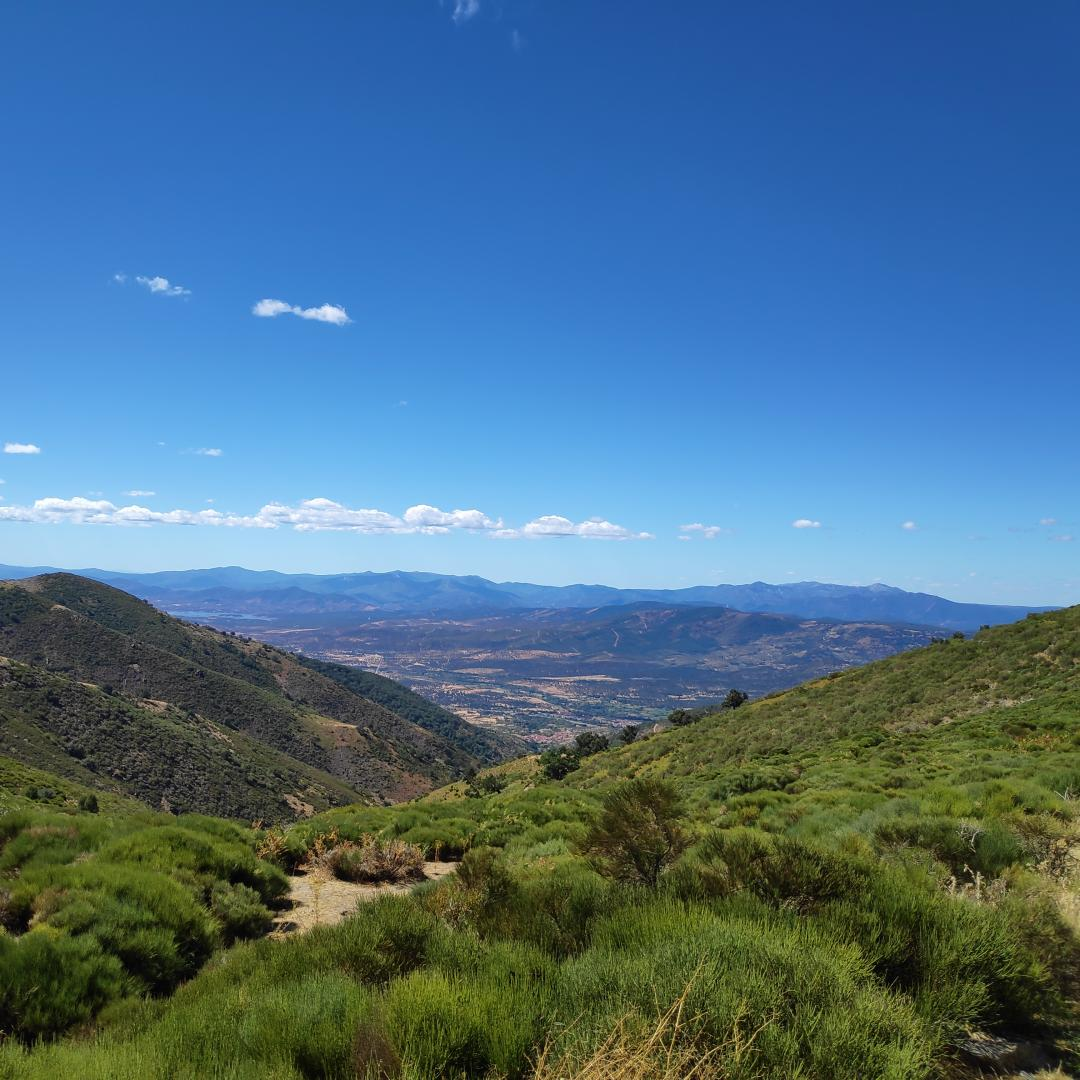
\includegraphics[width=0.65\textwidth]{imagenes/imagen2cuadro/propias/cezanne/IMG_20200830_161526_1.jpg}
            \end{subfigure}
        \hfill
            \begin{subfigure}[b]{0.49\textwidth}
            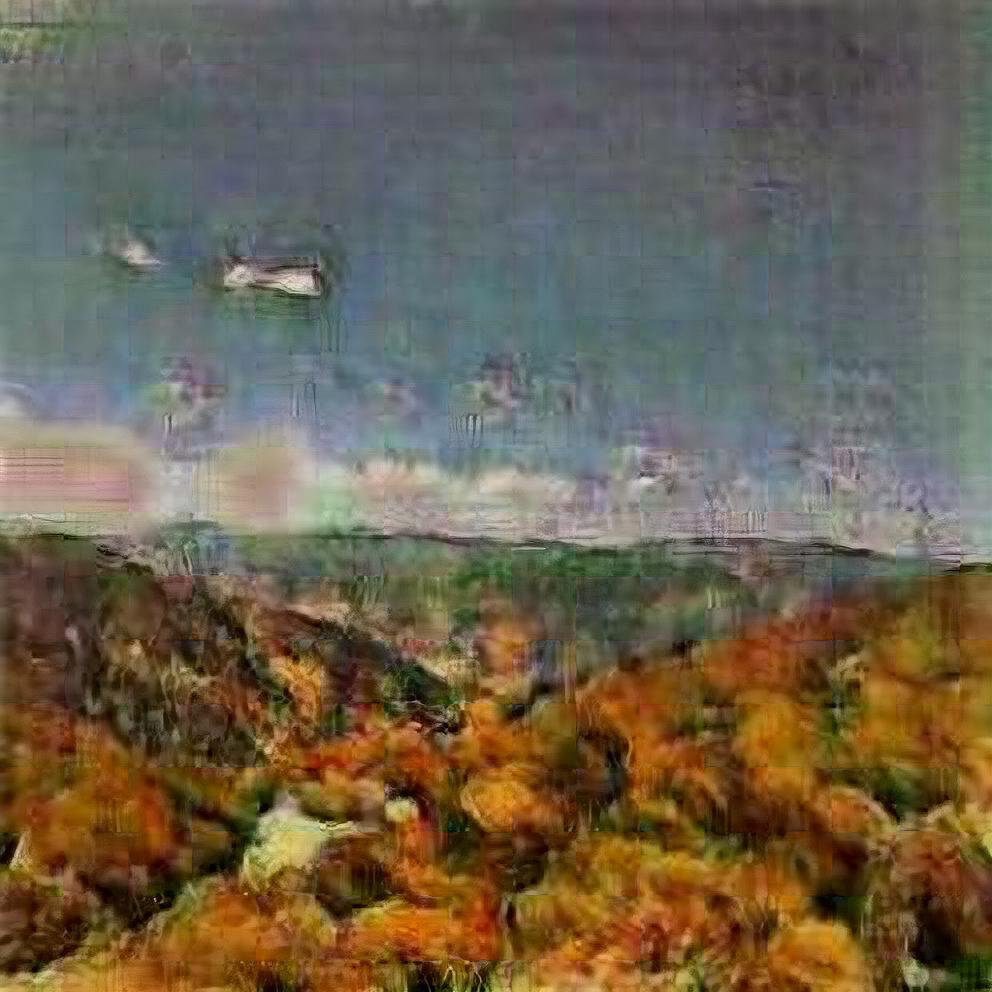
\includegraphics[width=0.65\textwidth]{imagenes/imagen2cuadro/propias/cezanne/IMG_20200830_161526_1_2.jpg}
            \end{subfigure}
        \caption{Cuadro de Cézanne generado de una foto en el puerto de Honduras (Cáceres)}
        \label{fig:cezanne_cuadro_puerto_honduras}
        \end{figure}
        
        \begin{figure}[!htb]
            \begin{subfigure}[b]{0.49\textwidth}
            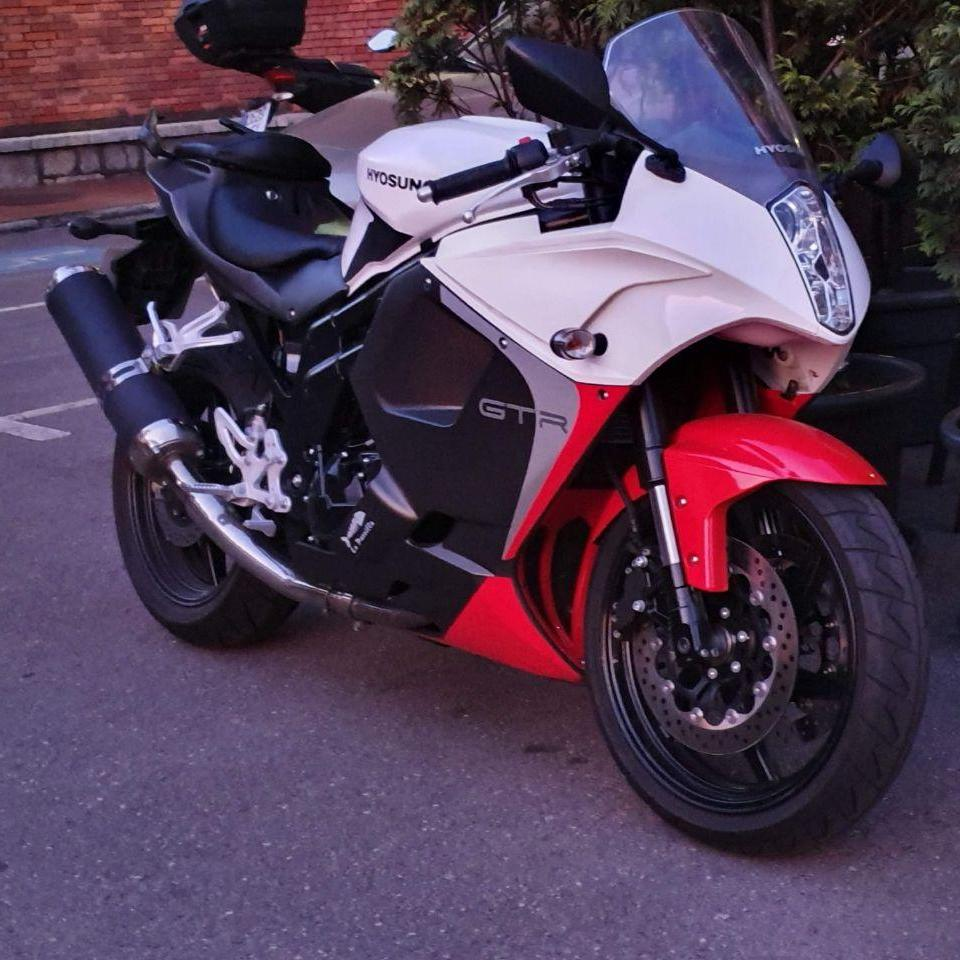
\includegraphics[width=0.65\textwidth]{imagenes/imagen2cuadro/propias/cezanne/photo_2020-10-23_16-29-18.jpg}
            \end{subfigure}
        \hfill
            \begin{subfigure}[b]{0.49\textwidth}
            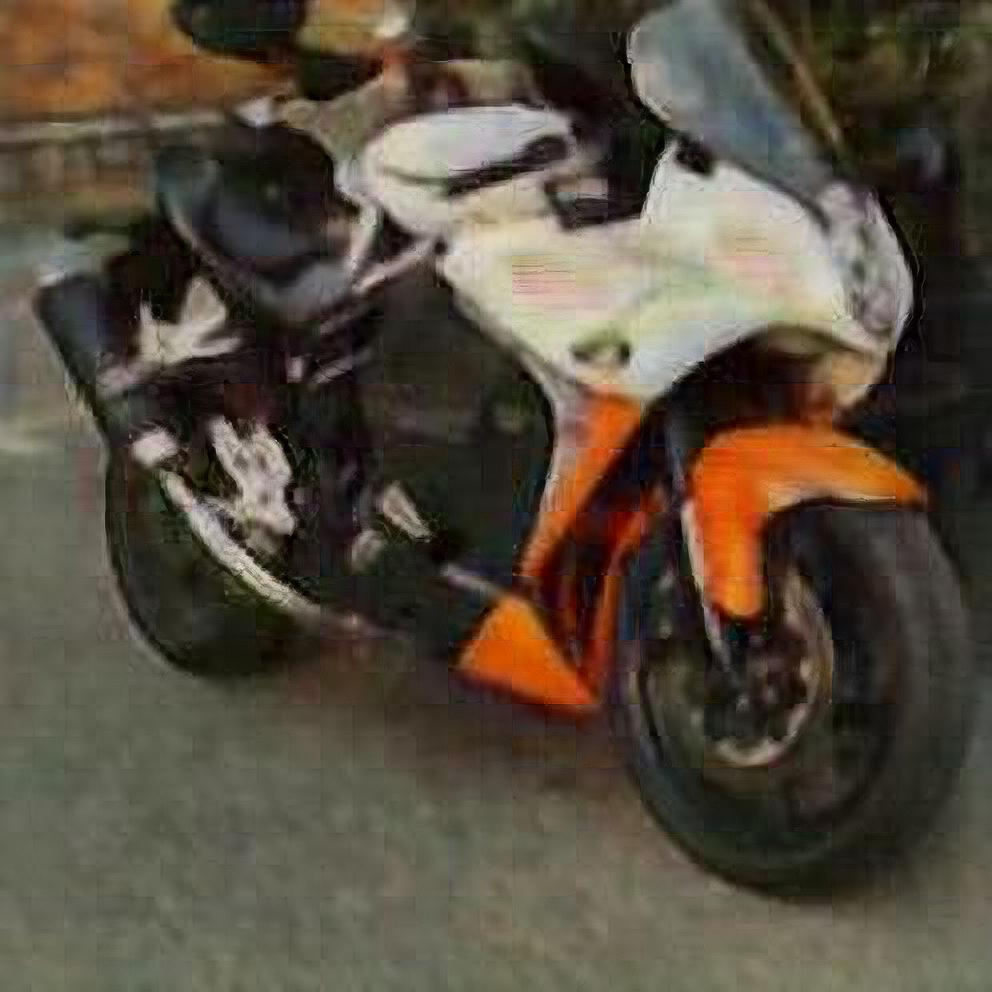
\includegraphics[width=0.65\textwidth]{imagenes/imagen2cuadro/propias/cezanne/photo_2020-10-23_16-29-18_2.jpg}
            \end{subfigure}
        \caption{Cuadro de Cézanne generado de una Hyosung GTR 650}
        \label{fig:cezanne_cuadro_moto_aparcada}
        \end{figure}
        
        En la figura \ref{fig:cezanne_cuadro_selfie_playa} puede verse el cambio de textura en la camisa, simplificándola; también puede apreciarse en la ilustración \ref{fig:cezanne_cuadro_arco_bcn}. Por otra parte es especialmente notable cómo cambian las texturas de los árboles y sus colores en las figuras \ref{fig:cezanne_cuadro_puerto_honduras} y \ref{fig:cezanne_cuadro_parque_madrid}, señal de que el sistema las ha aprendido con soltura.
        
        \newpage
    
    \paragraph{Monet}
    
    \begin{figure}[!htb]
            \begin{subfigure}[b]{0.49\textwidth}
            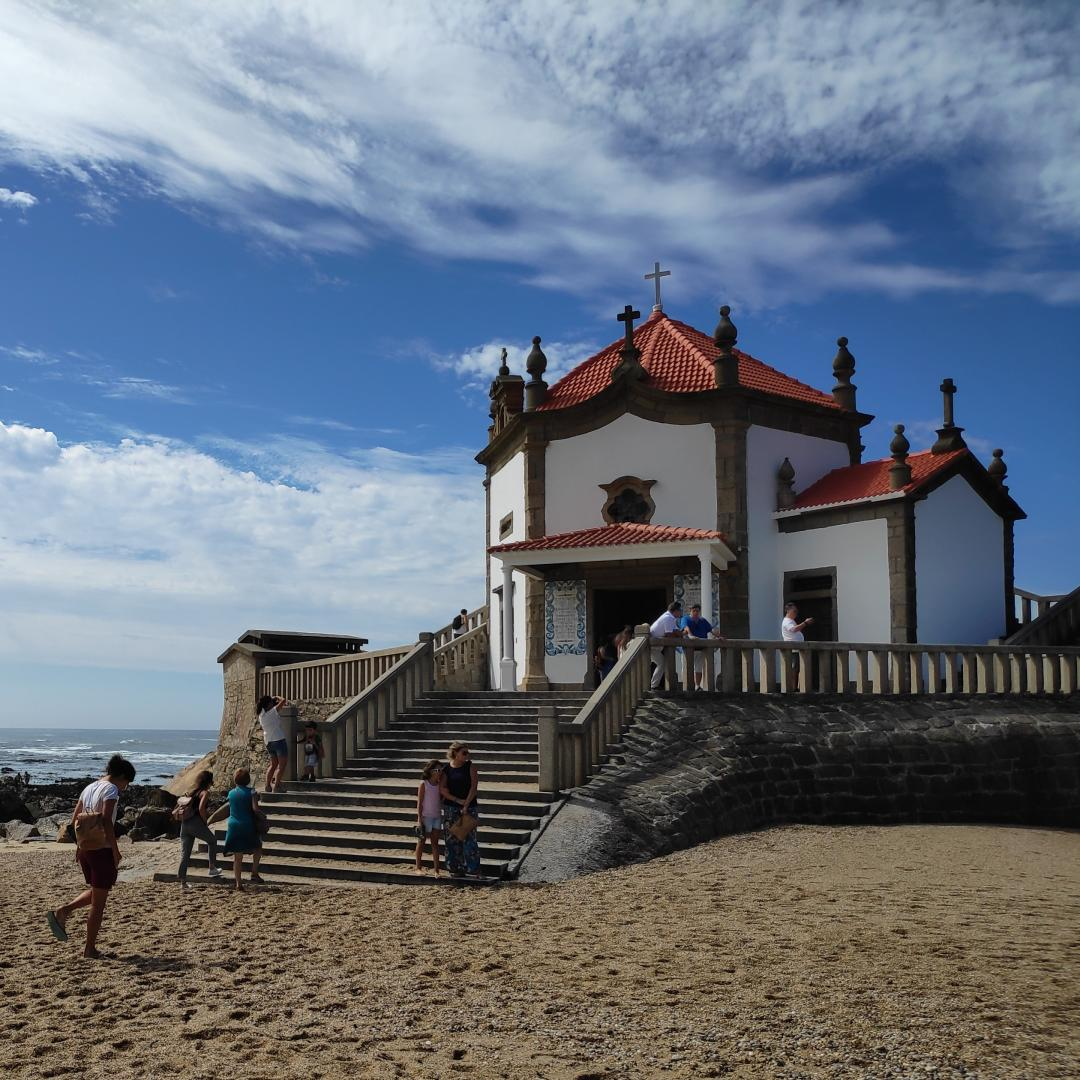
\includegraphics[width=0.65\textwidth]{imagenes/imagen2cuadro/propias/monet/IMG_20190901_131403.jpg}
            \end{subfigure}
        \hfill
            \begin{subfigure}[b]{0.49\textwidth}
            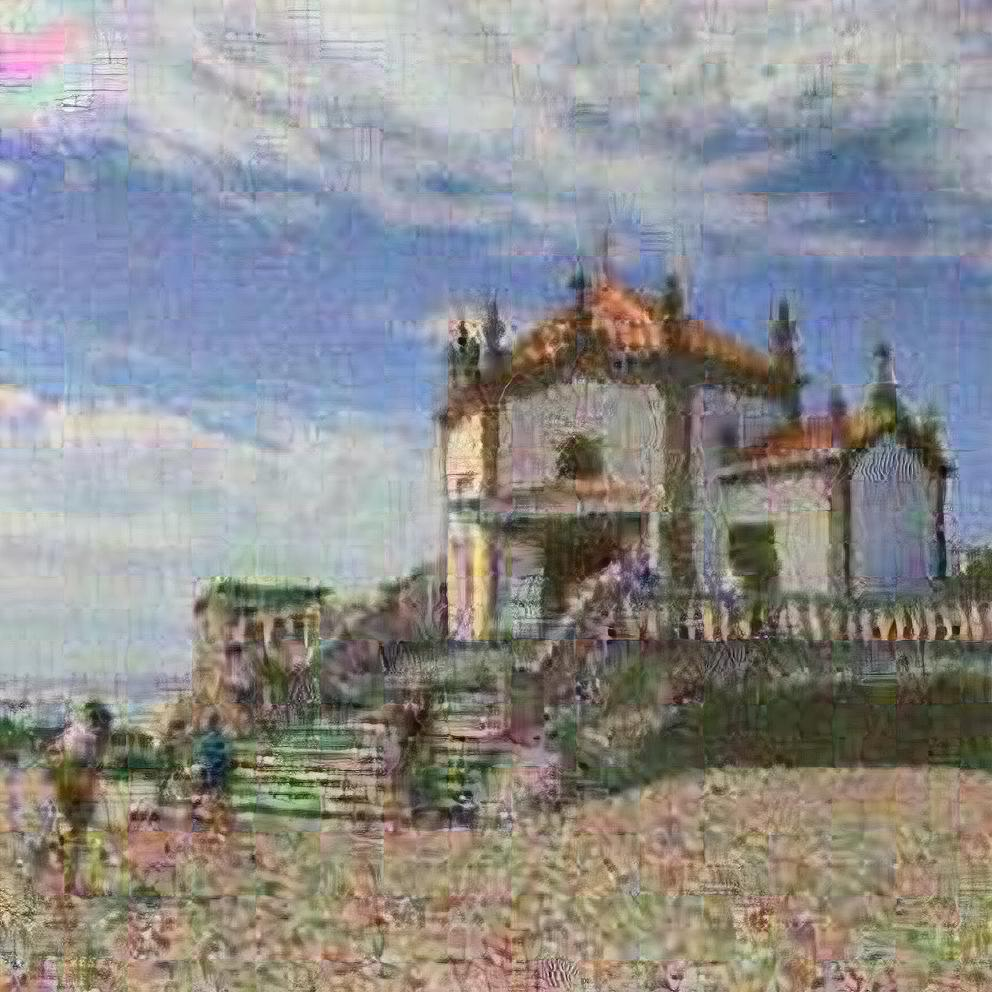
\includegraphics[width=0.65\textwidth]{imagenes/imagen2cuadro/propias/monet/IMG_20190901_131403_2.jpg}
            \end{subfigure}
        \caption{Cuadro de Monet generado a partir de una iglesia costera portuguesa}
        \label{fig:monet_cuadro_iglesia_portuguesa_playa}
        \end{figure}
        
        \begin{figure}[!htb]
            \begin{subfigure}[b]{0.49\textwidth}
            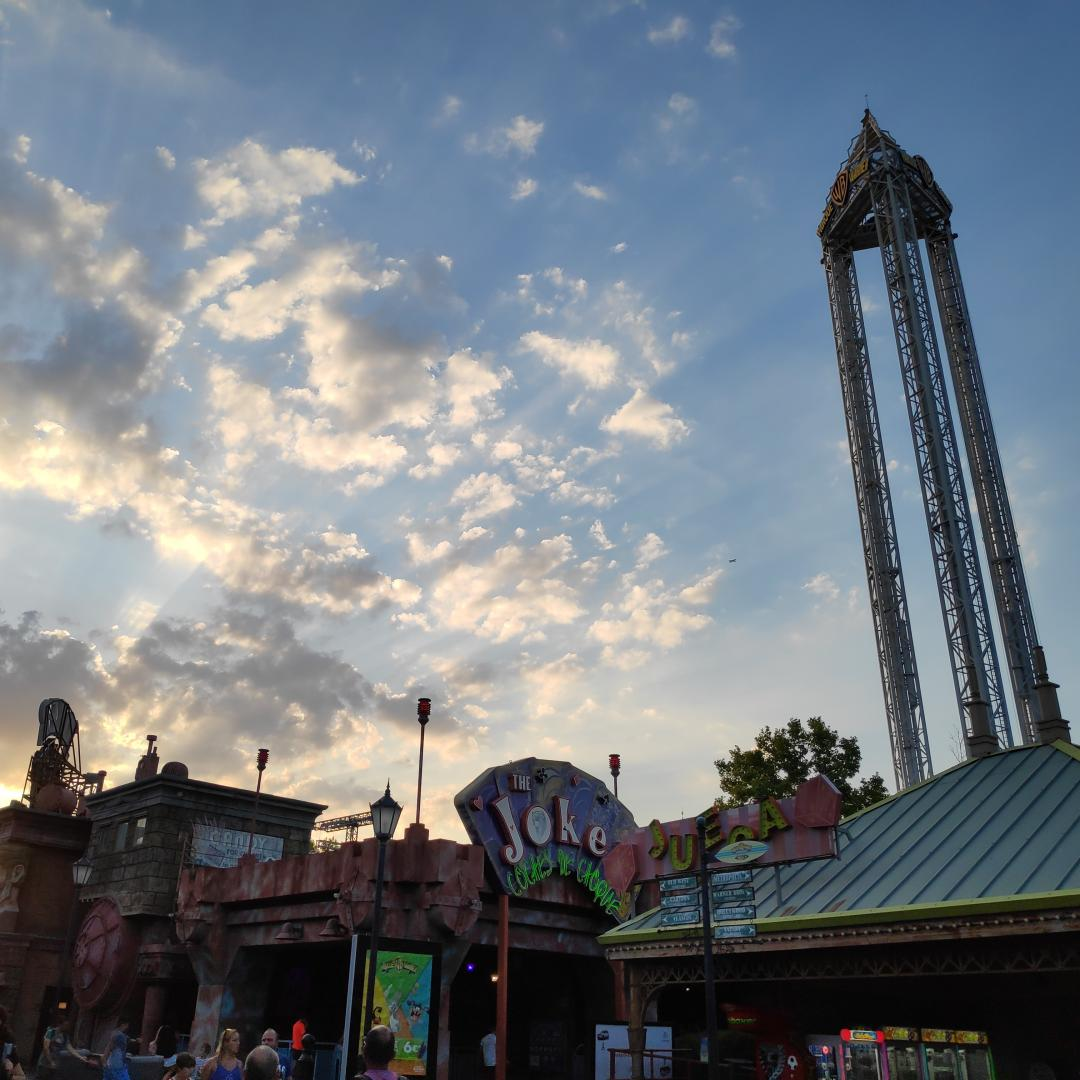
\includegraphics[width=0.65\textwidth]{imagenes/imagen2cuadro/propias/monet/IMG_20190903_200509.jpg}
            \end{subfigure}
        \hfill
            \begin{subfigure}[b]{0.49\textwidth}
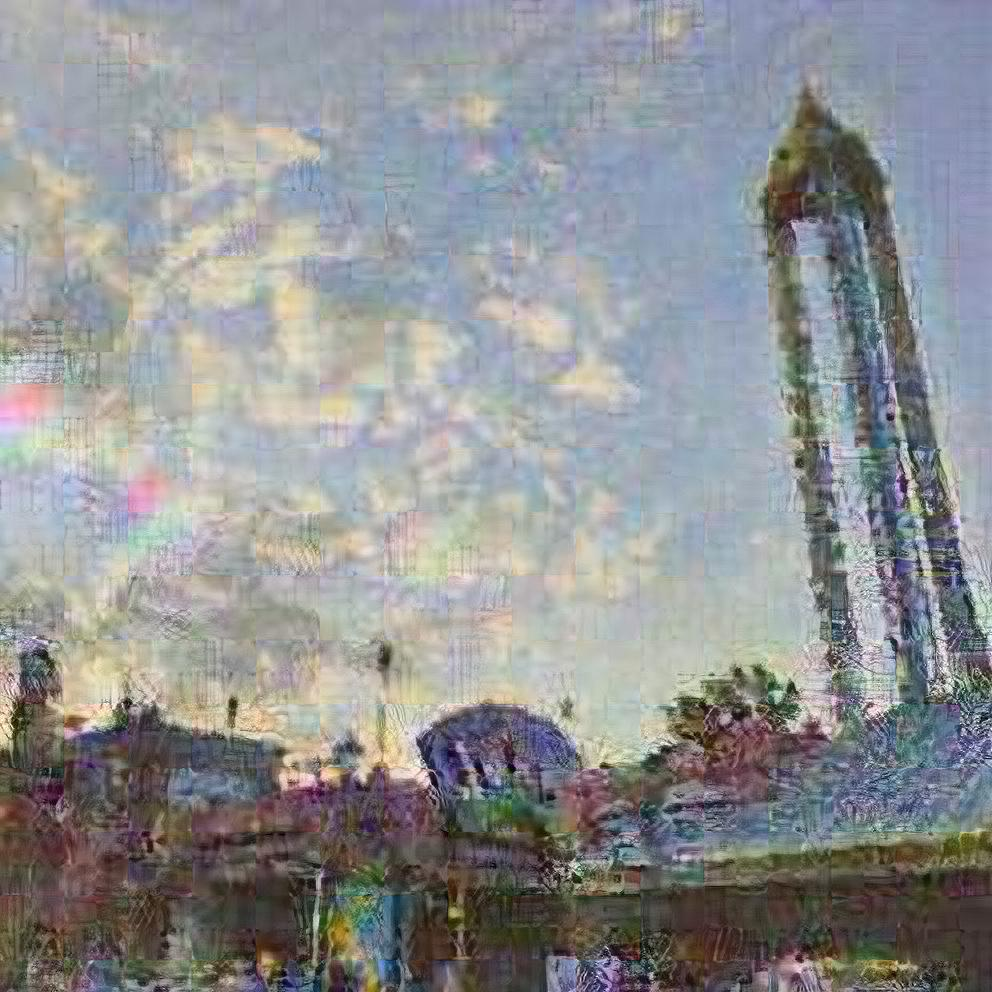
\includegraphics[width=0.65\textwidth]{imagenes/imagen2cuadro/propias/monet/IMG_20190903_200509_2.jpg}
            \end{subfigure}
        \caption{Cuadro de Monet generado en el parque Warner}
        \label{fig:monet_cuadro_warner}
        \end{figure}
        
        \begin{figure}[!htb]
            \begin{subfigure}[b]{0.49\textwidth}
            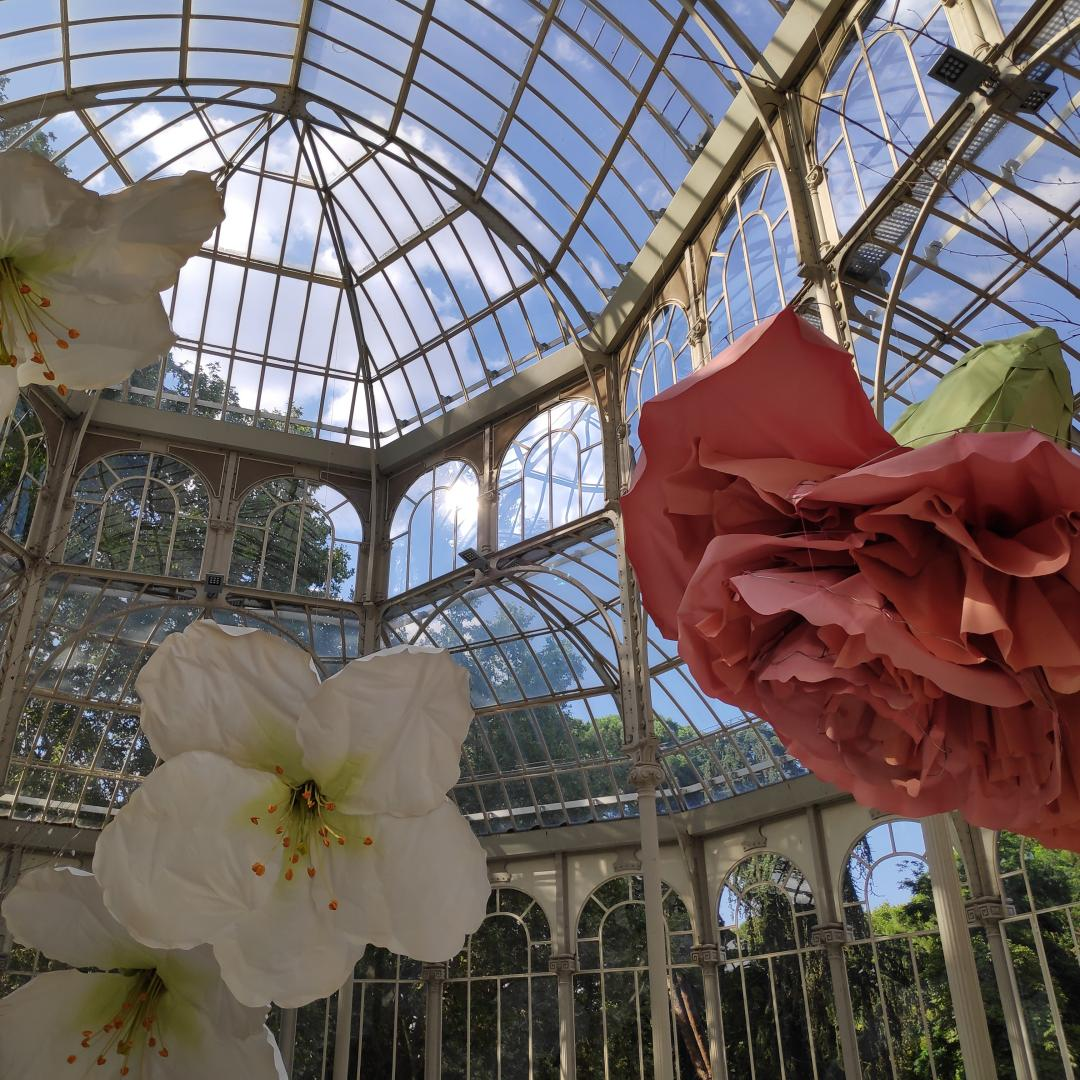
\includegraphics[width=0.65\textwidth]{imagenes/imagen2cuadro/propias/monet/IMG_20200722_184017_1.jpg}
            \end{subfigure}
        \hfill
            \begin{subfigure}[b]{0.49\textwidth}
            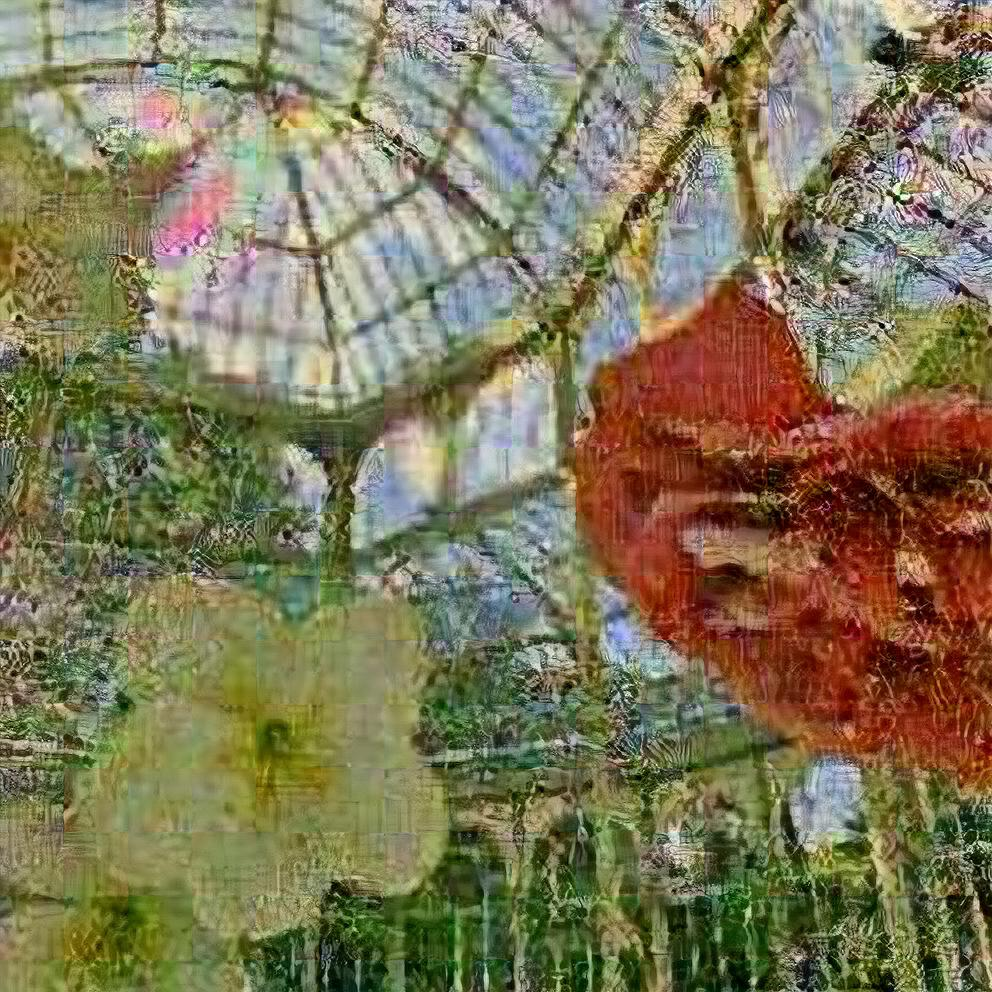
\includegraphics[width=0.65\textwidth]{imagenes/imagen2cuadro/propias/monet/IMG_20200722_184017_1_2.jpg}
            \end{subfigure}
        \caption{Cuadro de Monet generado en el Palacio de Cristal de Madrid}
        \label{fig:monet_cuadro_palacio_cristal}
        \end{figure}
        
        \begin{figure}[!htb]
            \begin{subfigure}[b]{0.49\textwidth}
            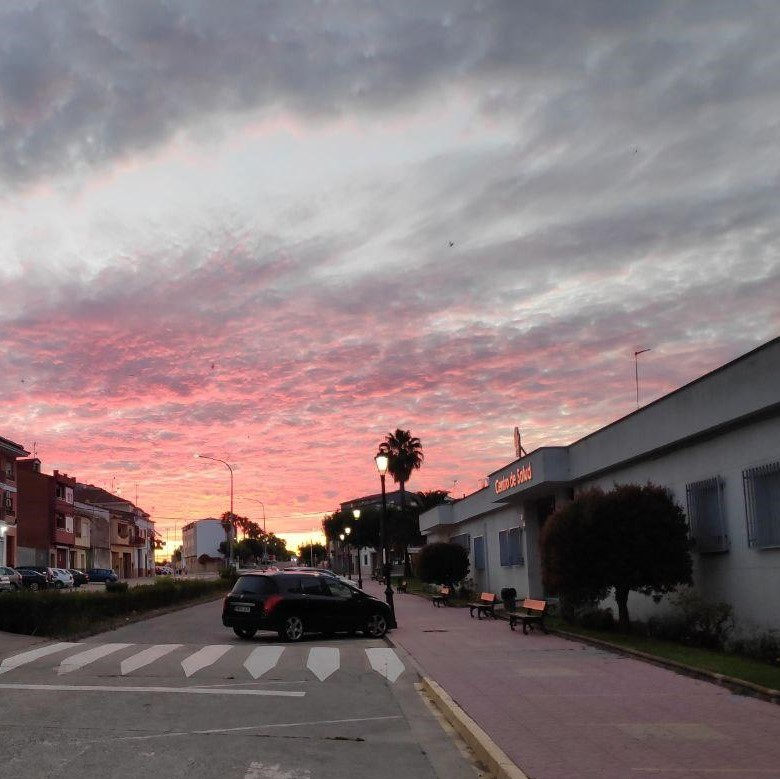
\includegraphics[width=0.65\textwidth]{imagenes/imagen2cuadro/propias/monet/photo_2020-07-01_21-19-44.jpg}
            \end{subfigure}
        \hfill
            \begin{subfigure}[b]{0.49\textwidth}
            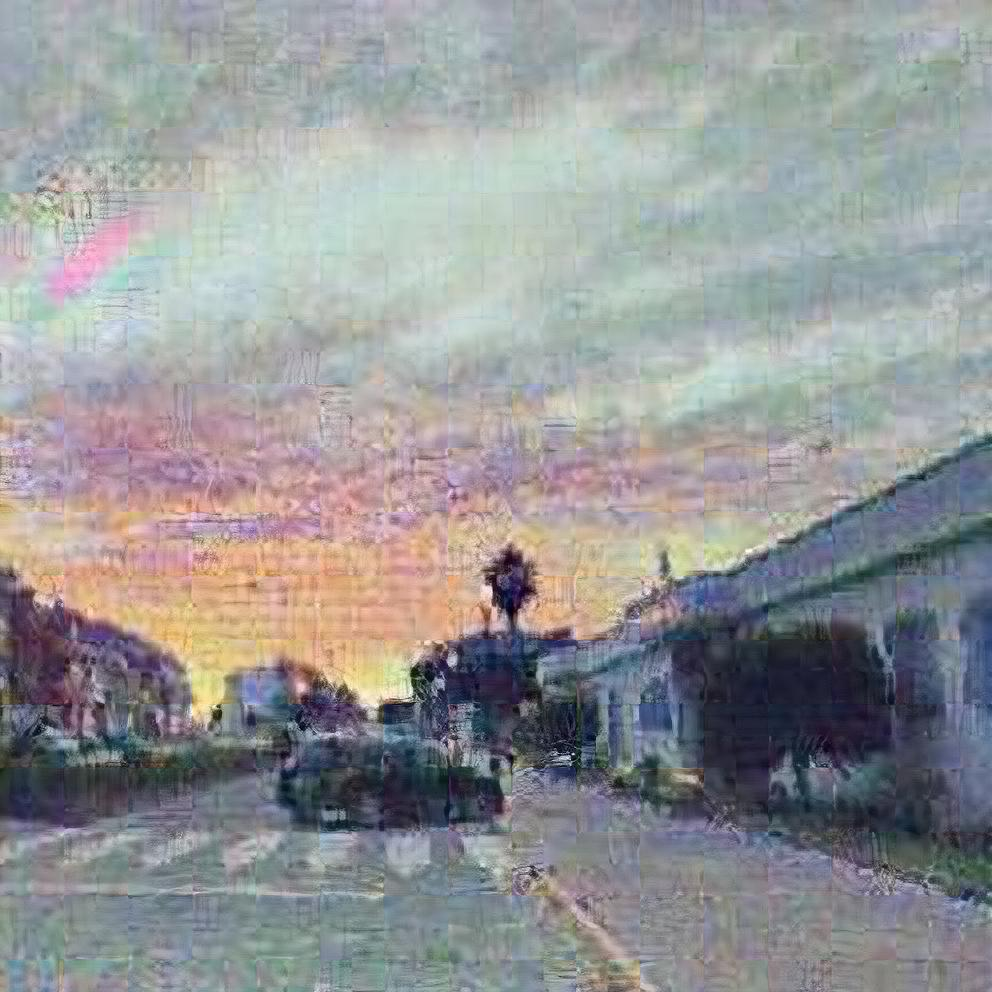
\includegraphics[width=0.65\textwidth]{imagenes/imagen2cuadro/propias/monet/photo_2020-07-01_21-19-44_2.jpg}
            \end{subfigure}
        \caption{Cuadro de Monet generado en el centro de salud de Montehermoso (Cáceres)}
        \label{fig:monet_cuadro_montehermoso}
        \end{figure}
        
        Se mantiene el impacto reducido de las transformaciones del modelo, señal de que el modelo quizás haya aprendido poco. Puede verse que los elementos que más mutan son el cielo y las estructuras metálicas de la ilustración \ref{fig:monet_cuadro_palacio_cristal}.
        
        \newpage
    
    \paragraph{Van Gogh}

    \begin{figure}[!htb]
            \begin{subfigure}[b]{0.49\textwidth}
            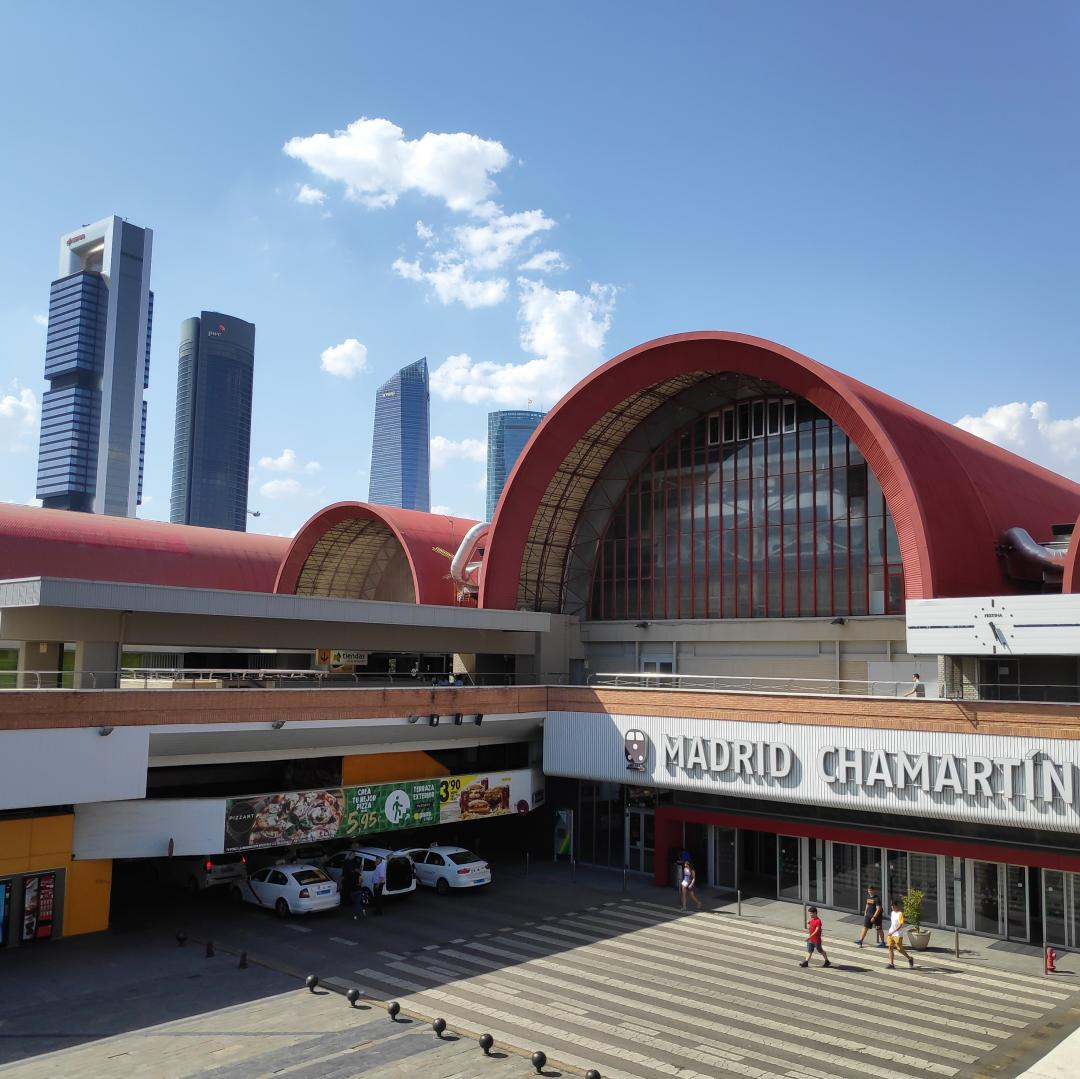
\includegraphics[width=0.65\textwidth]{imagenes/imagen2cuadro/propias/vangogh/IMG_20190724_172550_1.jpg}
            \end{subfigure}
        \hfill
            \begin{subfigure}[b]{0.49\textwidth}
            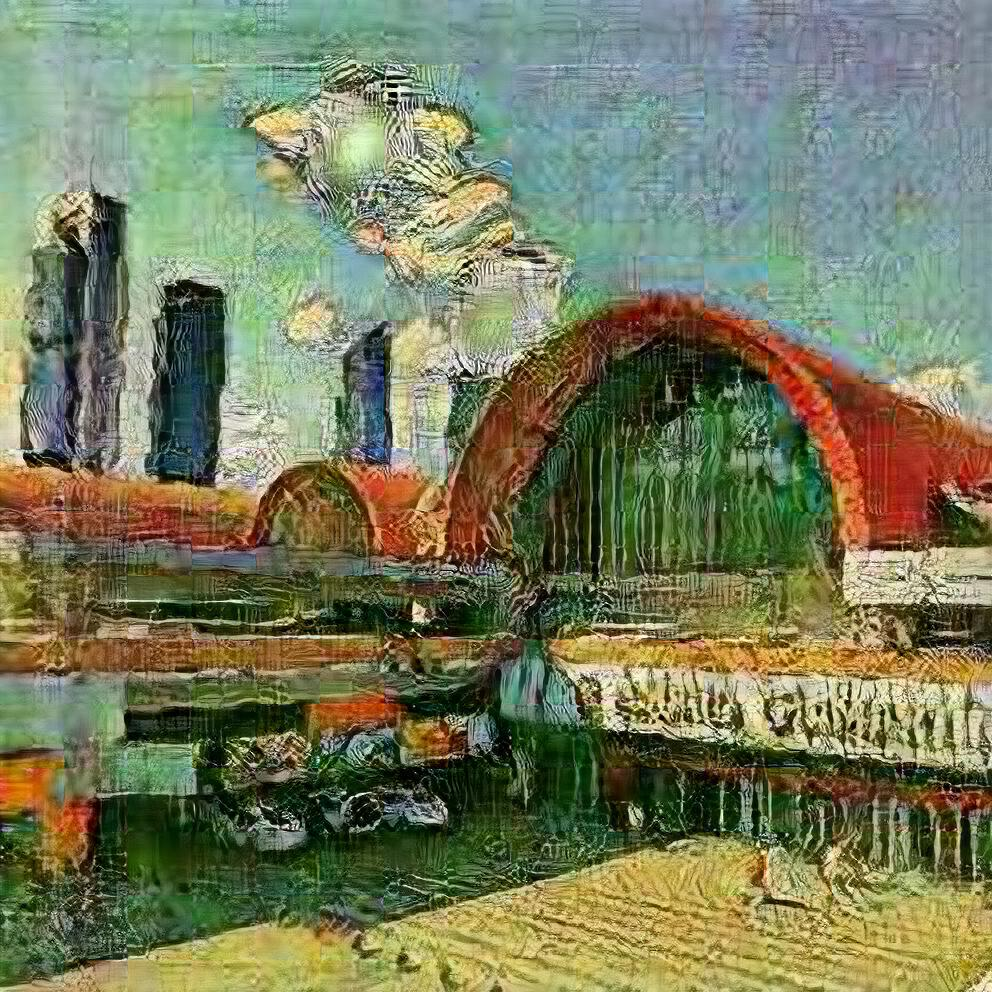
\includegraphics[width=0.65\textwidth]{imagenes/imagen2cuadro/propias/vangogh/IMG_20190724_172550_1_2.jpg}
            \end{subfigure}
        \caption{Cuadro de Van Gogh generado en la estación de Chamartín (Madrid)}
        \label{fig:vangogh_cuadro_chamartin}
        \end{figure}
        
        \begin{figure}[!htb]
            \begin{subfigure}[b]{0.49\textwidth}
            
\includegraphics[width=0.65\textwidth]{imagenes/imagen2cuadro/propias/vangogh/IMG_20200830_174622.jpg}
            \end{subfigure}
        \hfill
            \begin{subfigure}[b]{0.49\textwidth}
            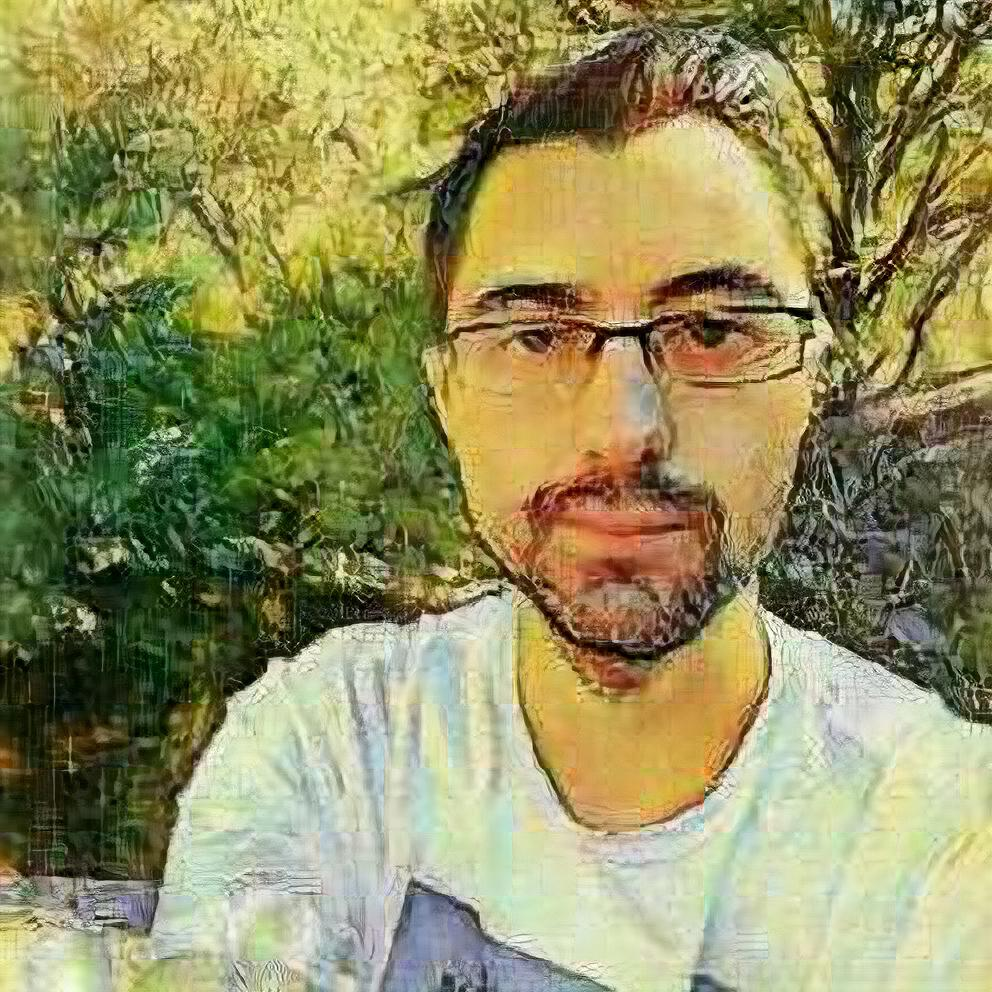
\includegraphics[width=0.65\textwidth]{imagenes/imagen2cuadro/propias/vangogh/IMG_20200830_174622_2.jpg}
            \end{subfigure}
        \caption{Cuadro de Van Gogh generado a partir de una foto del autor en Hervás (Cáceres)}
        \label{fig:vangogh_cuadro_hervas}
        \end{figure}
        
        \begin{figure}[!htb]
            \begin{subfigure}[b]{0.49\textwidth}
            
\includegraphics[width=0.65\textwidth]{imagenes/imagen2cuadro/propias/vangogh/photo_2020-07-01_21-19-51.jpg}
            \end{subfigure}
        \hfill
            \begin{subfigure}[b]{0.49\textwidth}
            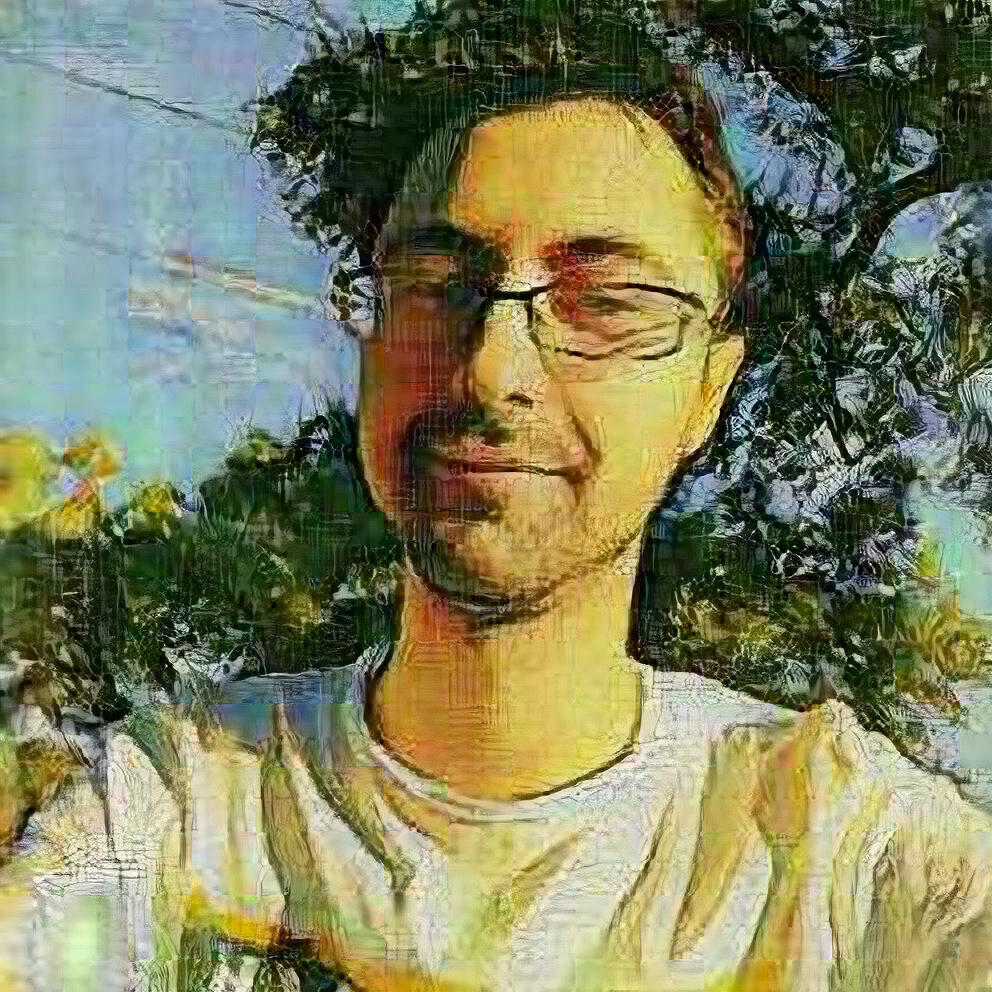
\includegraphics[width=0.65\textwidth]{imagenes/imagen2cuadro/propias/vangogh/photo_2020-07-01_21-19-51_2.jpg}
            \end{subfigure}
        \caption{Cuadro de Van Gogh generado a partir de una foto del autor en la Dehesa Boyal de Montehermoso (Cáceres)}
        \label{fig:vangogh_cuadro_dehesa}
        \end{figure}
        
        \begin{figure}[!htb]
            \begin{subfigure}[b]{0.49\textwidth}
            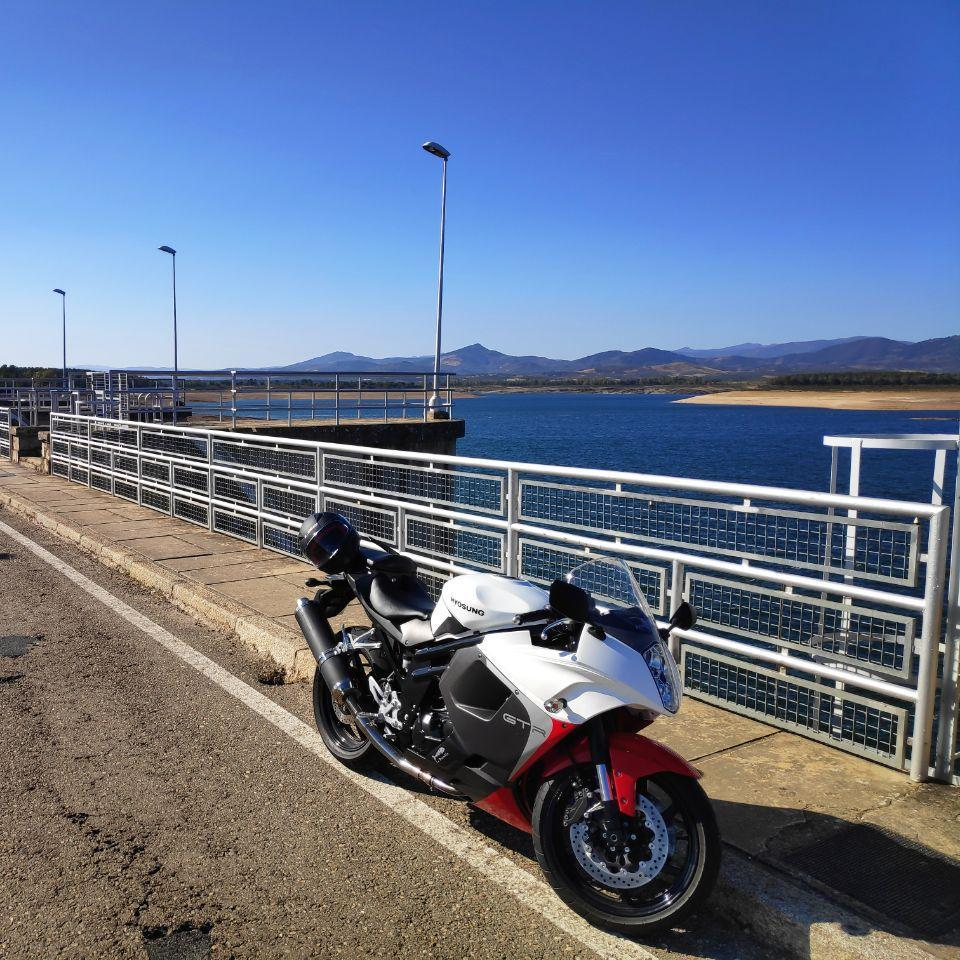
\includegraphics[width=0.65\textwidth]{imagenes/imagen2cuadro/propias/vangogh/photo_2020-10-23_16-26-00.jpg}
            \end{subfigure}
        \hfill
            \begin{subfigure}[b]{0.49\textwidth}
            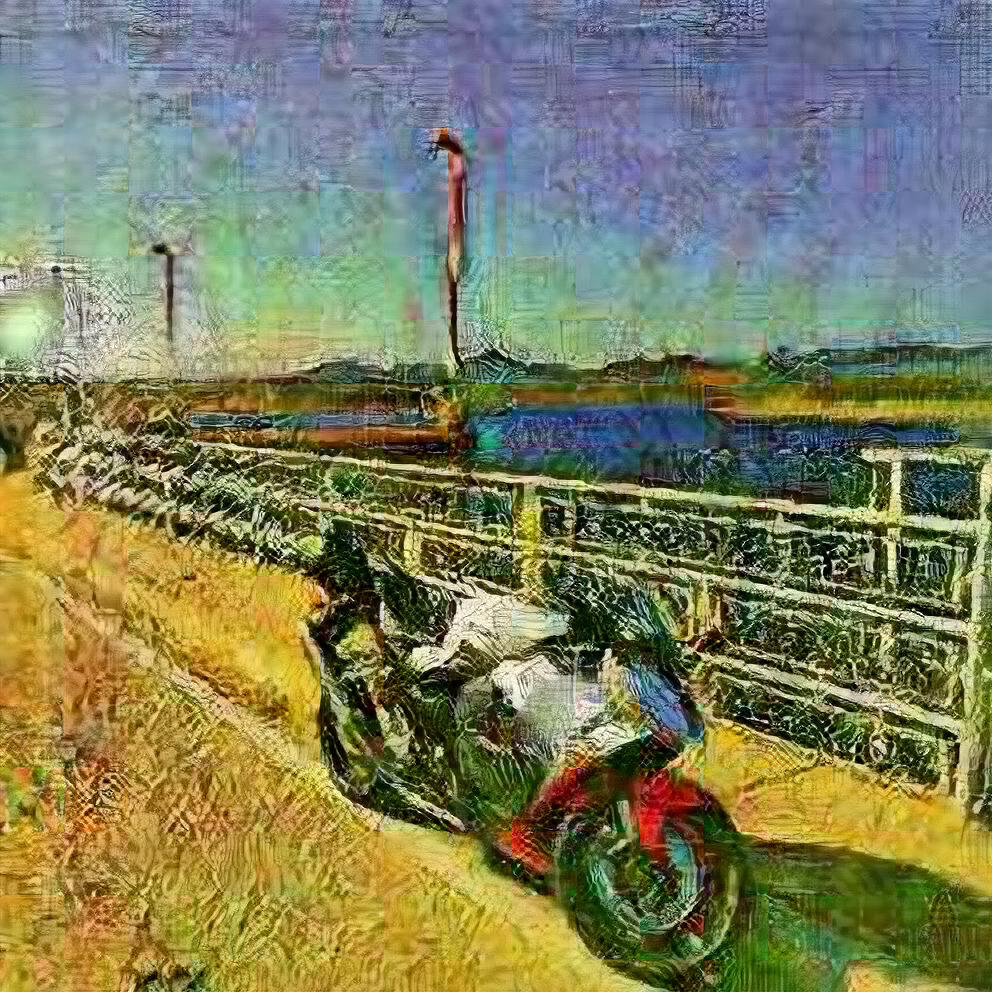
\includegraphics[width=0.65\textwidth]{imagenes/imagen2cuadro/propias/vangogh/photo_2020-10-23_16-26-00_2.jpg}
            \end{subfigure}
        \caption{Cuadro de Van Gogh a partir de una Hyosung GTR 650 estacionada en el pantano de Gabriel y Galán (Cáceres)}
        \label{fig:vangogh_cuadro_pantano_gabriel}
        \end{figure}
        
        Es especialmente notable el cambio de colores, dando paso a colores más chillones (figuras \ref{fig:vangogh_cuadro_hervas} y \ref{fig:vangogh_cuadro_dehesa}) y nuevamente las texturas (ilustración \ref{fig:vangogh_cuadro_chamartin}).
        
        \newpage

\subsection{Paso de cuadros a fotografías}

Si bien esta transformación no es objetivo del presente \tfg, se incluye como reflexión acerca de la transformación adicional que nos brinda el modelo Cycle GAN.

\subsubsection{Cézanne}

Puede verse en las figura \ref{fig:cezanne_foto_bouffan} y \ref{fig:cezanne_foto_landscape} que puede empezar a parecerse a una foto, ya que deshace relativamente bien la paleta de colores de Cézanne, pero sin embargo puede verse que los árboles son demasiado grandes y con errores gráficos, tapando las casas y generando por tanto una foto relativamente incorrecta (no olvidemos los planos superpuestos característicos de Cézanne, precursores del cubismo). \newline

Por último puede verse en la figura \ref{fig:cezanne_foto_pipa} que el modelo es realmente malo a la hora de trabajar con retratos pictóricos, dejando al hombre como una mera sombra.

\begin{figure}[!htb]
            \begin{subfigure}[b]{0.49\textwidth}
            \includegraphics[width=0.65\textwidth]{imagenes/cuadro2imagen/cezanne/00110.jpg}
            \end{subfigure}
        \hfill
            \begin{subfigure}[b]{0.49\textwidth}
            \includegraphics[width=0.65\textwidth]{imagenes/cuadro2imagen/cezanne/00110_2.jpg}
            \end{subfigure}
        \caption{Foto basada en el cuadro de Cézanne \textit{Marronniers et ferme au Jas de Bouffan}}
        \label{fig:cezanne_foto_bouffan}
        \end{figure}
        
        \begin{figure}[!htb]
            \begin{subfigure}[b]{0.49\textwidth}
            \includegraphics[width=0.65\textwidth]{imagenes/cuadro2imagen/cezanne/00230.jpg}
            \end{subfigure}
        \hfill
            \begin{subfigure}[b]{0.49\textwidth}
            \includegraphics[width=0.65\textwidth]{imagenes/cuadro2imagen/cezanne/00230_2.jpg}
            \end{subfigure}
        \caption{Foto basada en el cuadro de Cézanne \textit{Landscape. Study after Nature}}
        \label{fig:cezanne_foto_landscape}
        \end{figure}
        
        \begin{figure}[!htb]
            \begin{subfigure}[b]{0.49\textwidth}
            \includegraphics[width=0.65\textwidth]{imagenes/cuadro2imagen/cezanne/00570.jpg}
            \end{subfigure}
        \hfill
            \begin{subfigure}[b]{0.49\textwidth}
            \includegraphics[width=0.65\textwidth]{imagenes/cuadro2imagen/cezanne/00570_2.jpg}
            \end{subfigure}
        \caption{Foto basada en el cuadro de Cézanne \textit{Homme à la pipe}}
        \label{fig:cezanne_foto_pipa}
        \end{figure}
        
        \newpage

\subsubsection{Monet}

En el apartado anterior vimos que las transformaciones de Monet eran las menos agresivas, por lo que tiene sentido que las transformaciones inversas queden relativamente mejor que las de otros pintores. Podemos ver como aparece una paleta de colores con más contraste, especialmente en los tonos azules: mar de la figura \ref{fig:monet_foto_pourville} y cielo de las figuras \ref{fig:monet_foto_Argenteuil} y \ref{fig:monet_foto_Argenteuil}.

\begin{figure}[!htb]
            \begin{subfigure}[b]{0.49\textwidth}
            \includegraphics[width=0.65\textwidth]{imagenes/cuadro2imagen/monet/00010.jpg}
            \end{subfigure}
        \hfill
            \begin{subfigure}[b]{0.49\textwidth}
\includegraphics[width=0.65\textwidth]{imagenes/cuadro2imagen/monet/00010_2.jpg}
            \end{subfigure}
        \caption{Foto basada en el cuadro de Monet \textit{Callejón cerca de Pourville}}
        \label{fig:monet_foto_pourville}
        \end{figure}
        
        \begin{figure}[!htb]
            \begin{subfigure}[b]{0.49\textwidth}
            \includegraphics[width=0.65\textwidth]{imagenes/cuadro2imagen/monet/00900.jpg}
            \end{subfigure}
        \hfill
            \begin{subfigure}[b]{0.49\textwidth}
            \includegraphics[width=0.65\textwidth]{imagenes/cuadro2imagen/monet/00900_2.jpg}
            \end{subfigure}
        \caption{Foto basada en el cuadro de Monet \textit{The Promenade at Argenteuil}}
        \label{fig:monet_foto_Argenteuil}
        \end{figure}
        
        \begin{figure}[!htb]
            \begin{subfigure}[b]{0.49\textwidth}
            \includegraphics[width=0.65\textwidth]{imagenes/cuadro2imagen/monet/01010.jpg}
            \end{subfigure}
        \hfill
            \begin{subfigure}[b]{0.49\textwidth}
            \includegraphics[width=0.65\textwidth]{imagenes/cuadro2imagen/monet/01010_2.jpg}
            \end{subfigure}
        \caption{Foto basada en el cuadro de Monet \textit{El Verano}}
        \label{fig:monet_foto_verano}
        \end{figure}


\newpage

\subsubsection{Van Gogh}

Si bien quizás los cuadros de Van Gogh eran los que generaba mejor el modelo, vemos su contrapartida en esta parte: la foto de los girasoles (figura \ref{fig:vangogh_foto_girasoles}) es bastante irrealista, con colores antinaturales, y con abundantes errores de texturas en las figuras \ref{fig:vangogh_foto_zuecos} y \ref{fig:vangogh_foto_cypresse}.

        \begin{figure}[!htb]
            \begin{subfigure}[b]{0.49\textwidth}
            \includegraphics[width=0.6\textwidth]{imagenes/cuadro2imagen/vangogh/00002_2.jpg}
            \end{subfigure}
        \hfill
            \begin{subfigure}[b]{0.49\textwidth}
            \includegraphics[width=0.65\textwidth]{imagenes/cuadro2imagen/vangogh/00002.jpg}
            \end{subfigure}
        \caption{Foto basada en el cuadro de Van Gogh \textit{Un par de zuecos de cuero}}
        \label{fig:vangogh_foto_zuecos}
        \end{figure}
        
        \begin{figure}[!htb]
            \begin{subfigure}[b]{0.49\textwidth}
            \includegraphics[width=0.65\textwidth]{imagenes/cuadro2imagen/vangogh/00102.jpg}
            \end{subfigure}
        \hfill
            \begin{subfigure}[b]{0.49\textwidth}
            \includegraphics[width=0.65\textwidth]{imagenes/cuadro2imagen/vangogh/00102_2.jpg}
            \end{subfigure}
        \caption{Foto basada en el cuadro de Van Gogh \textit{Orchard Bordered by Cypresse}}
        \label{fig:vangogh_foto_cypresse}
        \end{figure}
        
        \begin{figure}[!htb]
            \begin{subfigure}[b]{0.49\textwidth}
            \includegraphics[width=0.65\textwidth]{imagenes/cuadro2imagen/vangogh/00180.jpg}
            \end{subfigure}
        \hfill
            \begin{subfigure}[b]{0.49\textwidth}
            \includegraphics[width=0.65\textwidth]{imagenes/cuadro2imagen/vangogh/00180_2.jpg}
            \end{subfigure}
        \caption{Foto basada en el cuadro de Van Gogh \textit{Jarrón con catorce girasoles}}
        \label{fig:vangogh_foto_girasoles}
        \end{figure}

\newpage

\section{Objetivos logrados}

El objetivo principal se ha podido ver que se ha cumplido, ya que el sistema funciona correctamente y se ha seguido una arquitectura con la que se pueden cambiar parámetros del modelo fácilmente. Artísticamente dista de emular fielmente el Impresionismo, pero podemos ver que con los avances en materia de redes de neuronas que se producen cada año quizás estemos más cerca de conseguirlo de lo que pueda parecer. \newline

Pasemos a hablar de los objetivos secundarios (cada punto se refiere al número de objetivo planteado):

\begin{enumerate}
    \item Dicha reflexión se ha realizado tanto en este apartado como en el capítulo conclusiones. 
    \item La implementación del modelo se ha realizado utilizando las herramientas más eficientes tanto de Python como de Keras y TensorFlow: 
        \begin{itemize}
            \item Python: uso del campo \textunderscore \textunderscore slots\textunderscore \textunderscore en la definición de las clases \cite{Chazallet}, ficheros .json de configuración del modelo, uso de la clase Pathlib para garantizar la compatibilidad entre sistemas operativos, patrones de diseño como Singleton para el ahorro de memoria, ficheros \textit{requirements.txt} especificando las dependencias del proyecto para ser instaladas con pip...
            \item Keras: uso de funciones para mostrar la arquitectura del modelo implementado y de la exportación de \textit{checkpoints} para restaurar el entrenamiento del modelo.
            \item TensorFlow: uso de su módulo \textit{Dataset} para la optimización de la lectura y el procesado de imágenes \cite{TensorFlow_Dataset}.
        \end{itemize}
   \item Para cambiar el dataset únicamente hay que indicarlo en los parámetros de lanzadera y realizar como máximo dos cambios en el fichero .json de configuración.
   \item Este objetivo se ha cumplido por completo al realizar los entrenos de la red utilizando instancias de cómputo y \textit{buckets} para el almacenamiento de los \textit{logs} en Google Cloud Platform.
   \item Gracias al \textit{microframework} Flask se ha cumplido este objetivo de forma muy sencilla e intuitiva: con una adaptación mínima podríamos desplegar el subsistema en un servidor externo y añadir nueva funcionalidad al mismo.
   \item El cumplimiento de este último objetivo es trivial al realizarse este documento desde 0, sin ninguna plantilla.
\end{enumerate}


\section{Problemas encontrados}
\begin{itemize}
    \item Imposibilidad de utilizar los pesos de la red EnhanceNet en otra implementación: este factor ha imposibilitado hacer más eficiente la propia implementación, además de no poder convertirla a TensorFlow 2, lo que ha forzado a utilizar versiones depreciadas de algunas librerías. 
    \item Entrenamiento de las redes CycleGAN muy costoso, lo que forzó a utilizar la instancia en Google Cloud Plataform con la promoción de nuevo usuario: entre 14 y 40h, según versiones en la instancia de la nube, entre 40 y 80 en el equipo del autor. Este factor limitante ha restringido enormemente la experimentación con el modelo, además de condicionar partes del diseño final de la propia implementación.
    \item Consumo elevado de recursos de GPU por parte del modelo, lo que ha limitado experimentos con la resolución de las imágenes.
    \item Dificultad de implementar y depurar la red. Debido a la complejidad intrínseca al modelo y a las peculiaridades de TensorFlow me resultó muy complicado hacer funcionar el modelo y depurar los errores en la transformación de imágenes.
    \item Métricas poco representativas: si bien los baremos de la función error de CycleGAN son comprensibles, cuesta extrapolarlos a las imágenes que arroja el modelo, lo que dificulta aún más la mejora del mismo.
    \item Documentación escasa para instalar correctamente CUDA y cuDNN.
\end{itemize}

\end{document}